
\documentclass[11pt]{article}
\usepackage[margin=0.95in]{geometry}
\usepackage{amsmath,amssymb,amsfonts,amsthm,mathtools}
\usepackage{booktabs,longtable,array,multirow}
\usepackage{enumitem}
\usepackage{graphicx}
\usepackage{xcolor}
\usepackage{hyperref}
\usepackage{tikz}
\usetikzlibrary{arrows.meta,positioning,fit,shapes,calc}
\usepackage{microtype}
\usepackage{fancyvrb}
\usepackage{titlesec}
\hypersetup{colorlinks=true,linkcolor=blue!50!black,citecolor=blue!50!black,urlcolor=blue!50!black}
\setlist[itemize]{leftmargin=1.25em,itemsep=0.15em,topsep=0.2em}
\setlist[enumerate]{leftmargin=1.45em,itemsep=0.15em,topsep=0.2em}
\newtheorem{theorem}{Theorem}[section]
\newtheorem{proposition}[theorem]{Proposition}
\newtheorem{lemma}[theorem]{Lemma}
\newtheorem{corollary}[theorem]{Corollary}
\theoremstyle{definition}
\newtheorem{definition}[theorem]{Definition}
\newtheorem{example}[theorem]{Example}
\newtheorem{objective}[theorem]{Objective}
\theoremstyle{remark}
\newtheorem{remark}[theorem]{Remark}
\newcommand{\T}{\mathbb{T}}
\newcommand{\R}{\mathbb{R}}
\newcommand{\Z}{\mathbb{Z}}
\newcommand{\N}{\mathbb{N}}
\newcommand{\C}{\mathbb{C}}
\newcommand{\K}{\mathbb{K}}
\newcommand{\F}{\mathbb{F}}
\newcommand{\val}{\operatorname{val}}
\newcommand{\Log}{\operatorname{Log}}
\newcommand{\Trop}{\operatorname{Trop}}
\newcommand{\Conv}{\operatorname{Conv}}
\newcommand{\argmax}{\operatorname*{arg\,max}}
\newcommand{\argmin}{\operatorname*{arg\,min}}
\newcommand{\softmax}{\operatorname{softmax}}
\newcommand{\sigmoid}{\operatorname{sigmoid}}
\newcommand{\CE}{\operatorname{CE}}
\newcommand{\KL}{\operatorname{KL}}
\newcommand{\Var}{\operatorname{Var}}
\newcommand{\Cov}{\operatorname{Cov}}
\newcommand{\E}{\mathbb{E}}
\newcommand{\Prob}{\mathbb{P}}
\newcommand{\Ind}{\mathbf{1}}
\newcommand{\dist}{\operatorname{dist}}
\newcommand{\rank}{\operatorname{rank}}
\newcommand{\Hom}{\operatorname{Hom}}
\newcommand{\im}{\operatorname{im}}
\newcommand{\oplusT}{\oplus}
\newcommand{\odotT}{\odot}
\newcommand{\loss}{\mathcal{L}}
\newcommand{\eps}{\varepsilon}
\newcommand{\traj}{\boldsymbol{\tau}}
\newcommand{\Prop}{\mathcal{P}}
\newcommand{\Ctx}{\mathfrak{C}}
\newcommand{\bits}{\operatorname{bits\mbox{-}per\mbox{-}byte}}
\newcommand{\norm}[1]{\left\lVert #1\right\rVert}
\newcommand{\abs}[1]{\left\lvert #1\right\rvert}
\newcommand{\ip}[2]{\left\langle #1,#2\right\rangle}
\newcommand{\trans}{^{\mathsf T}}
\numberwithin{equation}{section}
\sloppy
\title{\vspace{-1.5em}\textbf{TropicalGT IV: Tropical Oracle Trajectory Classifiers for Behavior, Reasoning Quality, and Bits-per-byte Control}}
\author{Amelie Schreiber}
\date{June 2026}

\begin{document}
\maketitle

\begin{abstract}
TropicalGT I introduced a graph-token reasoning model whose attention core can operate in the max-plus or min-plus semiring, exposing active supports, polyhedral margins, and dynamic-programming certificates while preserving bits-per-byte accountability. TropicalGT II lifted this local mechanism to iterative reasoning trajectories: standardized graph-of-thought packets, tropicalized hidden states, trajectory amoebas, patchworked reasoning charts, filtered simplicial persistence complexes, and ergodic cell summaries. TropicalGT III moved the same mathematics to the external substrate of modern agents: model-context-protocol traces, markdown memory, knowledge graphs, long-context windows, graph-structured vector databases, projected retrieval heads, tropical quantization, and context packing up to multi-million-token budgets.

This fourth paper adds an oracle layer.  The goal is to train either a compact additional head or a full oracle transformer that classifies partial and complete reasoning trajectories by properties that matter for deployment: correctness, verifier agreement, evidence grounding, proof rigor, tool discipline, compliance, safety, refusal appropriateness, tone, personality corridor, verbosity, calibration, efficiency, context-token utility, retrieval hygiene, memory freshness, and held-out bits-per-byte utility.  The oracle is not a post-hoc sentiment tagger.  It is a structured tropical classifier over graph-token trajectories and context graphs.  Its logits are piecewise-linear tropical polynomials; its label space is a property poset equipped with incompatibility complexes; its local judgments form a sheaf over trajectory windows; its control actions are computed by min-plus dynamic programming; and its deployment value is measured by downstream model improvement rather than oracle accuracy alone.

We develop definitions, theorem/proof statements, training losses, pseudocode, data schemas, ablations, and implementation protocols.  We prove equivariance, proper-scoring, side-information, tropical-margin, quantization-stability, Cech-gluing, Viterbi-control, monotone-policy-improvement, and bits-per-byte-gated promotion results under explicit finite or compact assumptions.  The paper is pragmatic: every classifier signal must either improve model behavior, lower error, reduce context waste, improve safety/compliance, improve style control, or produce a positive held-out bits-per-byte tradeoff after artifact and runtime costs.
\end{abstract}

\tableofcontents
\newpage

\section{Introduction}

The first three TropicalGT papers developed a structured training program for graph-token reasoning agents.  The first paper used tropical attention to expose max-plus supports and dynamic-programming structure.  The second paper treated repeated reasoning as a dynamical system of tropicalized packets and persistent complexes.  The third paper treated MCP traces, markdown memory, knowledge graphs, vector databases, and long-context windows as an external tropical context substrate.  These papers answer three questions: how should a reasoning step compute, how should a reasoning trajectory evolve, and how should an agent retrieve and assemble context.

A fourth question remains: how should the system know which trajectories are good?  A next-token loss evaluates a final byte stream.  A verifier checks only the task slice for which it was designed.  A safety classifier often sees only a final answer.  A retrieval metric may measure only top-k relevance.  None of these alone says whether the entire trajectory was accurate, grounded, efficient, compliant, calibrated, safe, properly toned, memory-hygienic, and context-efficient.  For that we need an oracle trajectory classifier.

\paragraph{The oracle problem.}
Let a base agent produce a trajectory
\begin{equation}
    \traj=(R_0,R_1,\ldots,R_T,y),
\end{equation}
where each packet \(R_t\) contains visible text, hidden summaries, graph-of-thought state, retrieved evidence, MCP or tool records, markdown-memory nodes, knowledge-graph neighborhoods, active tropical supports, verifier fields, and optional persistence or certificate data.  The oracle maps
\begin{equation}
    \mathcal O_\omega:\traj\longmapsto \hat p_\omega(\cdot\mid \traj)
\end{equation}
where the output is a calibrated distribution or score vector over trajectory properties.  Properties may be binary, ordinal, continuous, or structured.  Examples include \texttt{correct}, \texttt{grounded}, \texttt{unsafe-compliance}, \texttt{tool-relevant}, \texttt{memory-stale}, \texttt{tone-drift}, \texttt{too-verbose}, \texttt{proof-gap}, \texttt{context-waste}, and \texttt{answer-ready}.

\paragraph{Why tropical?}
Tropical attention is naturally suited to trajectory classification for three reasons.  First, many trajectory labels are dominated by worst-case or best-case events: one critical hallucinated citation, one unsafe tool call, one decisive proof gap, one high-quality evidence path, or one context block that makes the answer possible.  Max-plus and min-plus aggregation represent these extrema directly.  Second, tropical logits are piecewise-linear and have active supports, so the oracle can explain a label by the particular window, evidence block, tool event, or hidden cell that determined it.  Third, tropical margins make compression safe: if a label decision has a large margin, quantization or projection can preserve it.

\paragraph{The central thesis.}
A trajectory oracle is useful only if it changes model training or inference in a beneficial way.  It can filter low-quality data, weight supervised losses, construct preference pairs, shape GFlowNet rewards, reject bad graph-of-thought branches, gate MCP tool calls, prune stale memories, steer tone corridors, or stop long-context packing.  But its value is not its standalone F1 score.  Its value is downstream utility:
\begin{equation}
    U(\mathcal O)=\Delta \bits_{\rm heldout}+\lambda_A\Delta A+\lambda_R\Delta R+\lambda_C\Delta C-\rho_B\operatorname{bytes}(\mathcal O)-\rho_T\operatorname{latency}(\mathcal O),
\end{equation}
where \(A\) is task accuracy, \(R\) is reasoning/retrieval quality, and \(C\) is control reliability.  If \(U\le 0\), the oracle may remain teacher-side but should not be promoted into a deployed artifact.

\paragraph{Contributions.}
This paper contributes the following.
\begin{enumerate}
    \item It defines tropical trajectory-property classifiers for partial and complete graph-token reasoning traces.
    \item It gives two architectures: a compact oracle head on a frozen or jointly trained backbone, and a full oracle transformer over trajectory packets.
    \item It imposes structure on labels through property posets, incompatibility complexes, tropical property fans, local-window sheaves, calibration maps, and min-plus control graphs.
    \item It proves core guarantees under explicit assumptions: equivariance, tropical active-support stability, quantization safety, proper scoring, side-information bounds, sheaf gluing, Viterbi-optimal control, and oracle-guided policy improvement.
    \item It gives a practical training paradigm: data schema, label acquisition, weak supervision, verifier distillation, human calibration, synthetic perturbation generation, loss functions, pseudocode, ablations, deployment profiles, and reproducibility checklists.
    \item It provides an objective catalogue for improving reasoning accuracy, evidence grounding, behavior control, tone/personality stability, safety/compliance, long-context efficiency, and held-out bits-per-byte.
\end{enumerate}

\section{Continuity with TropicalGT I--III and the mathematical sources}

\subsection{Tropical attention as the local primitive}
The NeurIPS 2025 Tropical Attention paper introduces multi-head tropical attention as a max-plus attention mechanism for neural algorithmic reasoning.  It proves approximation results for tropical circuits and realizes tropical transitive closure through composition, explaining why the induced polyhedral decision boundaries remain sharp and scale-invariant rather than being smoothed by softmax \cite{hashemi2025openreview,hashemi2025arxiv}.  The released implementation includes a standalone tropical attention kernel and combinatorial algorithm tasks \cite{hashemi2025code}.  TropicalGT I used that mechanism as a graph-token primitive.

A max-plus head computes
\begin{equation}
    Y_{ic}=\max_j\{S_{ij}+V_{jc}\}.
\end{equation}
For classification, replace the output coordinate \(c\) by a property index \(p\).  The active set
\begin{equation}
    A_{ip}=\argmax_j\{S_{ij}+V_{jp}\}
\end{equation}
is a finite explanation: it identifies the token, window, evidence block, or certificate branch controlling the property score.  This is the central reason to use tropical structure for oracle labels.  It provides classifier explanations at the level of trajectory events rather than only feature saliency.

\subsection{Tropical geometry as global organization}
The attached tropical algebraic geometry resource introduces amoebas as logarithmic images of algebraic varieties, studies limits of rescaled amoebas, constructs non-Archimedean amoebas by valuations, defines the tropical semifield, defines tropical polynomials as maxima of affine functions, and defines tropical hypersurfaces as corner loci.  It also develops tropical curves with integer affine structure, balancing, Viro patchworking, and correspondence-style enumerative results.  These concepts gave TropicalGT II its language of trajectory amoebas, patchworked reasoning charts, balanced evidence flow, and ergodic cell occupation.

For TropicalGT IV, the relevant analogue is the \emph{property fan}.  A tropical oracle logit is
\begin{equation}
    g_p(\traj)=\max_{r\le R_p}\{b_{pr}+\langle a_{pr},\phi(\traj)\rangle\},
\end{equation}
where \(\phi(\traj)\) is a trajectory embedding or pooled packet representation.  The regions on which a single affine branch controls \(g_p\) form a polyhedral complex.  Boundaries between branches are tropical hypersurfaces.  When the class decision changes, the trajectory crosses a wall of this complex.  That wall should correspond to an interpretable event: evidence appeared, a proof gap closed, an unsafe request entered, a citation became stale, or a tone corridor was violated.

\subsection{TropicalGT III and the external context substrate}
TropicalGT III extended the theory from internal hidden trajectories to MCP traces, markdown memory, knowledge graphs, vector databases, graph-structured retrieval, projected retrieval heads, quantization, and long-context windows.  The external substrate was modeled as a valuated context graph whose nodes carry dense embeddings, tropical valuation vectors, quantized codes, provenance/security metadata, adjacency, and finite certificates.  Retrieval was treated as a tropical graph operation rather than a flat nearest-neighbor lookup.  The official MCP specification frames MCP as a protocol connecting LLM applications to external data sources and tools, and describes server-exposed tools with schemas and invocation metadata \cite{mcp2025spec,mcp2025tools}.  TropicalGT III turns those protocol events into graph nodes; TropicalGT IV classifies the trajectories that use them.

\subsection{The fourth iteration}
TropicalGT IV is therefore the classifier/control layer over the previous three levels.  The flow is:
\begin{equation}
\begin{aligned}
&\text{tropical attention}\rightarrow\text{trajectory dynamics}\rightarrow\text{context retrieval}\\
&\rightarrow\text{oracle trajectory typing}\rightarrow\text{improved training/control}.
\end{aligned}
\end{equation}
The oracle should see all relevant finite summaries but should not force private chain-of-thought exposure.  It may consume hidden summaries, active supports, evidence ids, verifier labels, tool schemas, context usage statistics, and final outputs.  User-visible reporting should expose concise rationales, citations, uncertainty, and verifier status, not raw hidden reasoning traces.

\begin{figure}[t]
\centering
\resizebox{0.96\textwidth}{!}{%
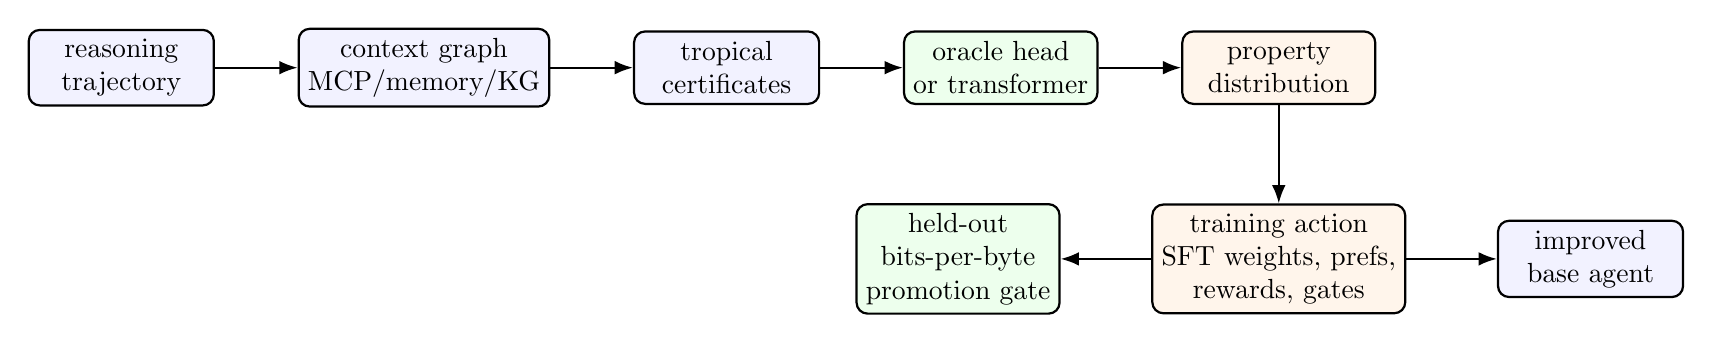
\begin{tikzpicture}[node distance=1.05cm,>=Latex,rounded corners,thick]
\tikzstyle{box}=[draw, rounded corners, align=center, minimum width=2.35cm, minimum height=0.92cm, fill=blue!5]
\tikzstyle{greenbox}=[draw, rounded corners, align=center, minimum width=2.35cm, minimum height=0.92cm, fill=green!7]
\tikzstyle{orangebox}=[draw, rounded corners, align=center, minimum width=2.45cm, minimum height=0.92cm, fill=orange!8]
\node[box] (traj) {reasoning\\trajectory};
\node[box, right=of traj] (ctx) {context graph\\MCP/memory/KG};
\node[box, right=of ctx] (cert) {tropical\\certificates};
\node[greenbox, right=of cert] (oracle) {oracle head\\or transformer};
\node[orangebox, right=of oracle] (labels) {property\\distribution};
\node[orangebox, below=1.25cm of labels] (action) {training action\\SFT weights, prefs,\\rewards, gates};
\node[greenbox, left=1.15cm of action] (gate) {held-out\\bits-per-byte\\promotion gate};
\node[box, right=1.15cm of action] (base) {improved\\base agent};
\draw[->] (traj.east) -- (ctx.west);
\draw[->] (ctx.east) -- (cert.west);
\draw[->] (cert.east) -- (oracle.west);
\draw[->] (oracle.east) -- (labels.west);
\draw[->] (labels.south) -- (action.north);
\draw[->] (action.east) -- (base.west);
\draw[->] (action.west) -- (gate.east);
\end{tikzpicture}}
\caption{TropicalGT IV system view.  The oracle reads trajectory packets, context events, and tropical certificates; predicts structured trajectory properties; and uses those predictions only through gated training or inference actions.}
\end{figure}

\section{Trajectory objects and property spaces}

\subsection{Trajectory packets}

\begin{definition}[Reasoning packet]
A reasoning packet is a tuple
\begin{equation}
    R_t=(G_t,H_t,X_t,C_t,E_t,V_t,A_t,B_t,M_t,U_t),
\end{equation}
where \(G_t\) is a typed graph-of-thought state, \(H_t\in\R^{n_t\times d}\) is a hidden summary table, \(X_t\) is visible text or a text pointer, \(C_t\subseteq \Ctx\) is the retrieved context subgraph, \(E_t\) is evidence/provenance metadata, \(V_t\) is verifier state, \(A_t\) is a tropical active-support certificate, \(B_t\) is an optional persistence or barcode summary, \(M_t\) is MCP/tool metadata, and \(U_t\) records behavior-control coordinates such as tone, verbosity, uncertainty, and safety-corridor features.
\end{definition}

\begin{definition}[Trajectory]
A trajectory is a finite sequence
\begin{equation}
    \traj=(R_0,R_1,\ldots,R_T,y)
\end{equation}
with final output \(y\).  A partial trajectory is \(\traj_{\le t}=(R_0,\ldots,R_t)\).  A trajectory is \emph{context-complete} for a task if the answer is expected to be derivable from the prompt, retrieved subgraphs, tool outputs, and generated intermediate states inside \(\traj\), subject to allowed inference rules.
\end{definition}

This object is intentionally more detailed than a transcript.  It makes explicit the hidden, retrieved, and audited pieces that a trajectory oracle may need.  In deployed privacy-preserving settings, the oracle can be trained or run on compressed summaries of these fields rather than raw private reasoning text.

\subsection{Property taxonomy}

Let \(\Prop=\{p_1,\ldots,p_m\}\) be a finite property set.  We distinguish five families.

\paragraph{Epistemic properties.} Correctness, verifier agreement, factual grounding, citation support, uncertainty calibration, proof rigor, contradiction absence, and evidence sufficiency.

\paragraph{Computational properties.} Efficiency, context-token utility, number of tool calls, latency, retrieval precision, retrieval closure quality, memory freshness, and bits-per-byte utility.

\paragraph{Behavioral properties.} Compliance, refusal appropriateness, safety-boundary respect, safe completion, unsafe compliance risk, and policy consistency.

\paragraph{Stylistic properties.} Tone corridor, personality profile stability, verbosity match, directness, uncertainty expression, didactic level, and user-intent adaptation.

\paragraph{Structural properties.} Stable active supports, large tropical margins, balanced evidence flow, patchworking gluing, persistence stability, ergodic non-thrashing, and context graph coherence.

\begin{definition}[Property poset]
A property poset is a finite partially ordered set \((\Prop,\preceq)\) where \(p\preceq q\) means that property \(q\) logically or operationally implies property \(p\).  For example, \texttt{fully-grounded} implies \texttt{partly-grounded}; \texttt{unsafe-compliance} implies \texttt{compliance-risk}; and \texttt{strict-proof-valid} implies \texttt{verifier-agreement} for a proof verifier under specified assumptions.
\end{definition}

\begin{definition}[Incompatibility complex]
An incompatibility complex is an abstract simplicial complex \(\Delta_{\Prop}\subseteq 2^\Prop\) whose faces are jointly compatible property sets.  Minimal nonfaces \(F\notin\Delta_{\Prop}\) encode forbidden simultaneous labels such as \(\{\texttt{fully-grounded},\texttt{unsupported-citation}\}\), \(\{\texttt{safe-refusal},\texttt{unsafe-compliance}\}\), or \(\{\texttt{concise-answer},\texttt{excessively-verbose}\}\).
\end{definition}

\begin{definition}[Label module]
A trajectory label is a vector \(y\in[0,1]^m\), an ordinal vector \(o\in\prod_j\{0,\ldots,K_j\}\), or a probability distribution over compatible subsets of \(\Prop\).  A label module is the graded vector space
\begin{equation}
    L=\bigoplus_{p\in\Prop} L_p
\end{equation}
whose coordinates are grouped by property family, severity, evidence type, and context-window location.
\end{definition}

The point of this structure is to prevent label independence from producing incoherent training.  A multi-label classifier that predicts both \texttt{properly-refuses} and \texttt{unsafe-compliance} with high confidence is not merely uncertain; it violates a known compatibility constraint.  A classifier that predicts \texttt{strict-proof-valid} but not \texttt{verifier-agreement} is similarly inconsistent unless the verifier is known to be incomplete.

\section{Tropical oracle architectures}

\subsection{Compact oracle head}

A compact oracle head is attached to a base TropicalGT or graph-token model.  Let \(\Phi_\theta\) be the base model and \(s_\theta(\traj)\in\R^d\) a pooled trajectory summary.  The summary may combine final hidden states, active-support histograms, verifier features, context usage statistics, and compressed evidence IDs:
\begin{equation}
    s_\theta(\traj)=\operatorname{Pool}\big(R_0,\ldots,R_T\big).
\end{equation}
For property \(p\), define a tropical logit
\begin{equation}
    g_p(\traj)=\max_{r\le R_p}\{b_{pr}+\langle a_{pr},s_\theta(\traj)\rangle\}.
\end{equation}
The probabilities are obtained by a calibration map, for instance
\begin{equation}
    \hat y_p=\sigmoid\left(\alpha_p g_p+\delta_p\right),
\end{equation}
for binary labels or a softmax over class logits for multiclass labels.

\begin{definition}[Tropical oracle head]
A tropical oracle head of rank \(R\) is a collection of piecewise-linear logits
\begin{equation}
    g_p(s)=\bigoplus_{r=1}^{R_p}\left(b_{pr}\odotT a_{pr}s\right)=\max_r\{b_{pr}+\langle a_{pr},s\rangle\},
\end{equation}
with active branch
\begin{equation}
    A_p(s)=\argmax_r\{b_{pr}+\langle a_{pr},s\rangle\}.
\end{equation}
Its explanation code is the tuple \((p,A_p(s),\Delta_p(s),W_p(s))\), where \(\Delta_p\) is the top-two margin and \(W_p\) is a pointer to the highest-contributing trajectory window.
\end{definition}

The compact head is the default first experiment.  It is cheap, easy to calibrate, and can be exported only if useful.  It is appropriate when labels can be predicted from pooled summaries.  It will fail when raw evidence spans, local tool schemas, or long-context ordering are decisive.

\subsection{Full oracle transformer}

A full oracle transformer reads the trajectory as a token sequence or graph.  The token types include packet summaries, message spans, retrieved blocks, MCP calls, tool outputs, knowledge-graph nodes, verifier judgments, active-support certificates, and behavior coordinates.  Attention can mix ordinary softmax heads with tropical heads.  Tropical heads are used for labels governed by extremal evidence: a single unsafe call, the best proof path, worst contradiction, strongest citation, or largest context-waste block.

\begin{definition}[Oracle transformer]
An oracle transformer is
\begin{equation}
    \mathcal O_\omega = D_\omega\circ \Psi_L\circ\cdots\circ \Psi_1\circ T_{\rm traj},
\end{equation}
where \(T_{\rm traj}\) tokenizes the trajectory object, \(\Psi_\ell\) are graph- or sequence-equivariant blocks with softmax and tropical heads, and \(D_\omega\) decodes property distributions, local-window labels, incompatibility warnings, and control actions.
\end{definition}

The full oracle is more expensive than a head.  It should usually be teacher-side.  It becomes deployment-relevant only when it can be distilled into a small head, a small set of tropical support codes, a retrieval gate, or a behavior-control adapter that passes the held-out bits-per-byte gate.

\subsection{Hybrid design}

In practice one trains a ladder.
\begin{enumerate}
    \item Frozen pooled head: train on existing trajectories with no base-model updates.
    \item Low-rank adapter head: allow a small projection of hidden states to specialize.
    \item Local-window oracle: add labels for short windows and tool/evidence events.
    \item Full oracle transformer: train as a teacher for hard labels.
    \item Distilled deployment head: export only useful property logits, gates, or low-rank controls.
\end{enumerate}

This ladder avoids a common failure: building a large judge model before proving that trajectory labels improve the base model.

\section{Tropical property fans and margin geometry}

\subsection{Property fans}

Let \(s\in\R^d\) be a trajectory summary.  For property \(p\), the tropical logit \(g_p(s)=\max_r\{b_{pr}+\langle a_{pr},s\rangle\}\) has a Newton polytope
\begin{equation}
    P_p=\Conv\{(a_{pr},b_{pr}):1\le r\le R_p\}\subset \R^{d+1}.
\end{equation}
The active branch is the exposed face of this lifted polytope under \((s,1)\).  The collection of regions with fixed active branch is a normal-fan-like polyhedral complex.

\begin{definition}[Property fan]
The property fan \(\Sigma_{\Prop}\) of an oracle head is the common refinement of the active-branch decompositions of all property logits \(g_p\), all pairwise class differences \(g_p-g_q\), and all incompatibility guard functions.  A chamber \(\sigma\in\Sigma_{\Prop}\) is a region of trajectory-summary space on which every tropical branch and every class ordering is fixed.
\end{definition}

\begin{proposition}[Polyhedrality of property chambers]
Every chamber of \(\Sigma_{\Prop}\) is an intersection of finitely many affine half-spaces.  In particular, it is a polyhedron.
\end{proposition}
\begin{proof}
For a fixed branch \(r\) of property \(p\) to be active, one requires
\begin{equation}
    b_{pr}+\langle a_{pr},s\rangle\ge b_{pu}+\langle a_{pu},s\rangle
\end{equation}
for every competing branch \(u\).  Each condition is an affine half-space.  Class orderings and guard inequalities are also finite affine comparisons once active branches are fixed.  A chamber is the intersection of all such finite conditions, hence a polyhedron.
\end{proof}

\begin{definition}[Trajectory-to-wall margin]
For a chamber \(\sigma\) containing \(s\), the property margin is
\begin{equation}
    \Delta_{\Prop}(s)=\min_{H\in\mathcal W(\sigma)} \frac{\operatorname{dist}_{\rm signed}(s,H)}{1+\norm{n_H}_2},
\end{equation}
where \(\mathcal W(\sigma)\) is the set of chamber walls and \(n_H\) is the wall normal.  The unnormalized tropical margin drops the denominator and uses the affine gap.
\end{definition}

Large margins mean the classifier is stable under small hidden-state perturbations, projection error, quantization, and minor context changes.  Small margins identify trajectories requiring escalation, more evidence, or full oracle processing.

\subsection{Tropical decision stability}

\begin{theorem}[Tropical active-branch stability]
Let \(g(s)=\max_r\{b_r+\langle a_r,s\rangle\}\).  Suppose branch \(r^\star\) is uniquely active at \(s\), and define the margin
\begin{equation}
    \Delta(s)=\min_{u\ne r^\star}\left[(b_{r^\star}-b_u)+\langle a_{r^\star}-a_u,s\rangle\right].
\end{equation}
If \(\norm{s-\tilde s}_2\le \eta\) and \(\eta\max_u\norm{a_{r^\star}-a_u}_2 < \Delta(s)/2\), then \(r^\star\) remains uniquely active at \(\tilde s\).
\end{theorem}
\begin{proof}
For any competitor \(u\), the active gap at \(\tilde s\) is
\begin{align}
(b_{r^\star}-b_u)+\langle a_{r^\star}-a_u,\tilde s\rangle
&=(b_{r^\star}-b_u)+\langle a_{r^\star}-a_u,s\rangle+\langle a_{r^\star}-a_u,\tilde s-s\rangle\\
&\ge \Delta(s)-\norm{a_{r^\star}-a_u}_2\norm{\tilde s-s}_2\\
&>\Delta(s)-\Delta(s)/2>0.
\end{align}
Thus every competitor remains strictly worse than \(r^\star\), so \(r^\star\) remains uniquely active.
\end{proof}

\begin{corollary}[Quantized oracle safety]
If a quantizer \(Q\) satisfies \(\norm{Q(s)-s}_2\le\eta\) and the margin condition of the theorem holds, then the quantized oracle has the same active branch and the same binary decision for every threshold whose distance from the logit is greater than the induced logit perturbation.
\end{corollary}

This result justifies storing compact oracle codes.  If an exported head is mostly used in high-margin regimes, int8 or product-quantized summaries can preserve decisions.  Low-margin cases should be escalated, not silently compressed.

\section{Structured oracle losses}

\subsection{Proper scoring and calibration}

The basic multi-label oracle loss is
\begin{equation}
    \loss_{\rm CE}= -\sum_{p\in\Prop}\left[y_p\log \hat y_p+(1-y_p)\log(1-\hat y_p)\right].
\end{equation}
For ordinal labels, use cumulative-link or threshold losses.  For continuous labels, use Gaussian, beta, or quantile losses depending on the scale.  Cross-entropy alone is not enough; the oracle must be calibrated because thresholds for safety, refusal, or escalation depend on probabilities.

\begin{theorem}[Binary cross-entropy is strictly proper]
Let \(Y\in\{0,1\}\) with \(\Prob(Y=1\mid X)=p(X)\).  Among predictions \(q(X)\in(0,1)\), the conditional expected binary cross-entropy
\begin{equation}
    \ell(q;p)= -p\log q-(1-p)\log(1-q)
\end{equation}
 is uniquely minimized at \(q=p\).
\end{theorem}
\begin{proof}
Differentiate with respect to \(q\):
\begin{equation}
    \frac{\partial \ell}{\partial q}= -\frac{p}{q}+\frac{1-p}{1-q}.
\end{equation}
Setting this to zero gives \(p(1-q)=(1-p)q\), hence \(q=p\).  The second derivative is \(p/q^2+(1-p)/(1-q)^2>0\), so the minimizer is unique.
\end{proof}

\subsection{Poset isotonicity}

If \(p\Rightarrow q\) in the property poset, then \(\hat y_p\le \hat y_q\) or \(\hat y_q\le\hat y_p\) depending on convention.  We fix the convention \(p\preceq q\) means \(q\) implies \(p\), so \(\hat y_p\ge \hat y_q\).  The isotonic penalty is
\begin{equation}
    \loss_{\rm iso}=\sum_{p\preceq q}\left[\hat y_q-\hat y_p\right]_+^2.
\end{equation}

\begin{proposition}[Projection to the isotonic cone]
Let
\begin{equation}
    \mathcal C_{\rm iso}=\{z\in\R^m:z_p\ge z_q\text{ whenever }p\preceq q\}.
\end{equation}
The Euclidean projection \(\Pi_{\mathcal C_{\rm iso}}(u)\) exists, is unique, and is nonexpansive.
\end{proposition}
\begin{proof}
The set \(\mathcal C_{\rm iso}\) is a closed convex cone because it is an intersection of finitely many closed half-spaces \(z_p-z_q\ge 0\).  Projection onto a nonempty closed convex subset of a Hilbert space exists and is unique.  The projection map onto a closed convex set is firmly nonexpansive, hence nonexpansive.
\end{proof}

During inference one may project raw logits or probabilities to \(\mathcal C_{\rm iso}\) before making decisions.  During training, the differentiable penalty encourages the same structure without solving a projection at every step.

\subsection{Incompatibility penalties}

Let \(\mathcal F_{\min}\) be the minimal nonfaces of \(\Delta_\Prop\).  The Stanley-Reisner-style incompatibility penalty is
\begin{equation}
    \loss_{\rm inc}=\sum_{F\in\mathcal F_{\min}}\prod_{p\in F}\hat y_p.
\end{equation}
This penalty is high only when all properties in a forbidden set are simultaneously high.  A log-sum-exp softened variant is
\begin{equation}
    \loss_{\rm inc}^{\tau}=\sum_{F\in\mathcal F_{\min}}\tau\log\left(1+\exp\left(\frac{\sum_{p\in F}\log(\hat y_p+\eps)-\kappa_F}{\tau}\right)\right).
\end{equation}

\begin{lemma}[Minimal nonface gradients concentrate on joint violations]
For \(F\in\mathcal F_{\min}\), the gradient of \(\prod_{p\in F}\hat y_p\) with respect to \(\hat y_q\) is \(\prod_{p\in F\setminus\{q\}}\hat y_p\) if \(q\in F\), and zero otherwise.
\end{lemma}
\begin{proof}
This is the elementary product rule.  Variables outside \(F\) do not appear.  For \(q\in F\), differentiating the product removes the factor \(\hat y_q\) and leaves all other factors.
\end{proof}

Thus the penalty does not waste gradient on non-violating labels.  It acts most strongly when the rest of a forbidden combination is already high.

\subsection{Tropical margin and active-support losses}

For a property branch margin \(\Delta_p(\traj)\), define
\begin{equation}
    \loss_{\rm margin}=\sum_{p\in\Prop} w_p\,[\gamma_p-\Delta_p(\traj)]_+^2.
\end{equation}
For a label with teacher support \(A_p^\star\), define an active-support loss
\begin{equation}
    \loss_{\rm support}=\sum_p \CE\left(\operatorname{onehot}(A_p^\star),\operatorname{softmax}(\ell_{p1},\ldots,\ell_{pR_p})\right),
\end{equation}
where \(\ell_{pr}=b_{pr}+\langle a_{pr},s\rangle\).  This teaches not only what label to assign but why the label was assigned.

\subsection{Sheaf gluing over trajectory windows}

A trajectory can be covered by windows \(U_i=[t_i,t_i+\ell]\).  The oracle produces local labels \(s_i\in\mathcal F(U_i)\).  Overlaps should agree unless a property genuinely changes.

\begin{definition}[Trajectory label presheaf]
Let \(\mathcal U\) be a cover of a trajectory index set \(\{0,\ldots,T\}\).  A label presheaf \(\mathcal F\) assigns to each window \(U\in\mathcal U\) a vector space or probability simplex \(\mathcal F(U)\) of local property judgments, and to each inclusion \(V\subset U\) a restriction map \(\rho_{UV}:\mathcal F(U)\to\mathcal F(V)\).
\end{definition}

The gluing loss is
\begin{equation}
    \loss_{\rm glue}=\sum_{i<j}\norm{\rho_{U_i,U_i\cap U_j}s_i-\rho_{U_j,U_i\cap U_j}s_j}_2^2.
\end{equation}

\begin{theorem}[Finite sheaf gluing criterion]
Assume \(\mathcal F\) is a sheaf of vector spaces on a finite trajectory cover and \(\{s_i\in\mathcal F(U_i)\}\) satisfies \(\rho_{U_i,U_i\cap U_j}s_i=\rho_{U_j,U_i\cap U_j}s_j\) for all overlaps.  Then there is a unique global section \(s\in\mathcal F(\cup_i U_i)\) restricting to every \(s_i\).
\end{theorem}
\begin{proof}
This is the sheaf gluing axiom specialized to a finite cover.  Existence follows because pairwise-compatible local sections glue to a section on the union; uniqueness follows from the locality axiom: if two global sections have identical restrictions to every element of the cover, they are equal.
\end{proof}

For neural training, the loss does not assert exact sheaf behavior.  It supplies a local-to-global regularizer: a trajectory should not be labeled \texttt{grounded} on one window and \texttt{unsupported} on an overlapping window without an explicit event explaining the transition.

\subsection{Composite objective}

The default oracle training objective is
\begin{align}
\loss_{\rm oracle}={}&\loss_{\rm CE}+\lambda_{\rm iso}\loss_{\rm iso}+\lambda_{\rm inc}\loss_{\rm inc}+\lambda_{\rm margin}\loss_{\rm margin}+\lambda_{\rm support}\loss_{\rm support}\nonumber\\
&+\lambda_{\rm glue}\loss_{\rm glue}+\lambda_{\rm cal}\loss_{\rm cal}+\lambda_{\rm byte}\loss_{\rm byte}+\lambda_{\rm distill}\loss_{\rm distill}.
\end{align}
The byte term penalizes large exported codes and long oracle rationales.  The calibration term can be expected calibration error, Brier score, temperature-scaled validation NLL, or slice calibration over property families.

\section{Oracle-guided training and control}

\subsection{From labels to training actions}

The oracle produces actions, not merely labels.  Common actions are:
\begin{enumerate}
    \item discard or downweight low-quality training trajectories;
    \item construct preference pairs from high-quality and low-quality completions;
    \item shape GFlowNet or search rewards;
    \item gate tool calls or require additional verification;
    \item restrict retrieval to fresh, grounded, permission-compatible memory;
    \item adjust decoding style through low-rank behavior vectors;
    \item stop context packing when marginal utility is negative;
    \item escalate low-margin or high-risk cases to full oracle or human review.
\end{enumerate}

\subsection{Side information and bits-per-byte}

A central question is why oracle labels can improve compression.  If the oracle output \(Z=\mathcal O(\traj)\) is predictive of future bytes \(X\), then conditioning on \(Z\) can lower log loss.  The following standard information-theoretic identity is the cleanest statement.

\begin{theorem}[Side-information log-loss improvement]
Let \(X\) be held-out text and \(Z\) an oracle signal available before predicting \(X\).  The optimal expected log-loss improvement from conditioning on \(Z\), measured in bits, is
\begin{equation}
    H_2(X)-H_2(X\mid Z)=I_2(X;Z),
\end{equation}
where \(H_2\) and \(I_2\) use base-2 logarithms.  Per byte, the maximum expected improvement is \(I_2(X;Z)/\E|X|_{\rm bytes}\) when lengths are deterministic or after the corresponding length-normalized conditioning.
\end{theorem}
\begin{proof}
The optimal code without side information uses \(p(x)\) and has expected length \(H_2(X)\).  The optimal code with side information uses \(p(x\mid z)\) and has expected length \(H_2(X\mid Z)\).  Their difference is the mutual information identity \(I_2(X;Z)=H_2(X)-H_2(X\mid Z)\).
\end{proof}

The theorem is not a guarantee that a learned oracle improves bits-per-byte.  It says the available improvement is exactly the predictive information that survives training, quantization, and deployment costs.  This is why oracle labels should be selected for downstream predictivity, not subjective appeal.

\subsection{Bayes thresholds for risk properties}

\begin{proposition}[Cost-sensitive threshold]
Let \(p=\Prob(Y=1\mid\traj)\) be a calibrated risk probability.  If blocking a safe trajectory has cost \(C_{\rm FP}\) and allowing a risky trajectory has cost \(C_{\rm FN}\), the Bayes action is to block when
\begin{equation}
    p>\frac{C_{\rm FP}}{C_{\rm FP}+C_{\rm FN}}.
\end{equation}
\end{proposition}
\begin{proof}
Allowing has expected cost \(pC_{\rm FN}\).  Blocking has expected cost \((1-p)C_{\rm FP}\).  Block when \((1-p)C_{\rm FP}<pC_{\rm FN}\), which rearranges to the stated inequality.
\end{proof}

This proposition is why calibration is not cosmetic.  A miscalibrated oracle produces wrong risk thresholds even if its ranking performance is high.

\subsection{Min-plus behavior control}

Some control decisions are sequential.  For example, a long-context answer may pass through states \texttt{retrieve}, \texttt{tool-call}, \texttt{verify}, \texttt{summarize}, \texttt{answer}, with costs for tone drift, risk, latency, and context bytes.  This is a shortest-path problem in a control graph.

\begin{definition}[Behavior-control graph]
A behavior-control graph is a directed graph \(\mathcal B=(Q,E)\) whose vertices are control states and whose edges \(q\to q'\) have costs
\begin{equation}
    c_t(q,q')=c_{\rm task}+c_{\rm risk}+c_{\rm tone}+c_{\rm byte}+c_{\rm latency}-c_{\rm evidence}.
\end{equation}
The best control path for a trajectory prefix is the min-plus dynamic program
\begin{equation}
    D_{t+1}(q')=\min_{q:q\to q'}\{D_t(q)+c_t(q,q')\}.
\end{equation}
\end{definition}

\begin{theorem}[Tropical oracle implements finite-horizon control]
For a finite behavior-control graph with bounded costs, a min-plus tropical attention block with edge masks can compute one Bellman relaxation exactly, and a stack of \(T\) such blocks computes the finite-horizon optimal control values.
\end{theorem}
\begin{proof}
For each target state \(q'\), mask keys to predecessor states \(q\) with edges \(q\to q'\).  Store candidate values \(D_t(q)+c_t(q,q')\).  A min-plus head computes their minimum, which is exactly the Bellman update.  Repeating the block \(T\) times computes the dynamic program by induction on horizon.
\end{proof}

\subsection{Oracle-guided policy improvement}

Let \(\pi\) be a trajectory-generating policy and let \(Q^{\mathcal O}(\traj,a)\) be an oracle-estimated action value for a training action or reasoning move.  Use it for reward shaping only if it is calibrated and if off-policy evaluation passes.

\begin{proposition}[Conservative oracle improvement]
Assume a finite action space and a calibrated lower confidence bound \(\underline Q(\traj,a)\le Q^\star(\traj,a)\) with probability at least \(1-\delta\) uniformly over candidate actions.  If a new policy \(\pi'\) is obtained by choosing only actions whose lower confidence bound exceeds the baseline action value by at least \(\eta>0\), then with probability at least \(1-\delta\), every changed decision improves true value by at least \(\eta\).
\end{proposition}
\begin{proof}
On the event that all lower bounds are valid, \(\underline Q(\traj,a)\le Q^\star(\traj,a)\).  The decision rule changes from baseline action \(a_0\) to \(a\) only when \(\underline Q(\traj,a)\ge Q^\star(\traj,a_0)+\eta\) or when a lower bound for the baseline is included with the corresponding conservative comparison.  Therefore \(Q^\star(\traj,a)\ge \underline Q(\traj,a)\ge Q^\star(\traj,a_0)+\eta\).  The probability statement follows from the assumed simultaneous confidence event.
\end{proof}

This is deliberately conservative.  It prevents a beautiful but unreliable oracle from steering the base model aggressively.

\section{Label acquisition and weak supervision}

\subsection{Label sources}

Trajectory labels can come from several sources, each with different reliability.
\begin{enumerate}
    \item Exact task checkers: unit tests, math answer checkers, theorem provers, graph algorithms, symbolic calculators.
    \item Verifiers: citation checkers, proof checkers, tool-call schema checkers, retrieval-grounding checkers.
    \item Human rubrics: tone, helpfulness, refusal appropriateness, uncertainty expression, and personality corridor.
    \item Synthetic perturbations: inject stale memories, remove citations, corrupt tool outputs, add irrelevant context, alter tone, or create contradiction pairs.
    \item Cross-model judges: teacher models label difficult qualitative properties, followed by calibration and bias audits.
    \item Self-consistency and multiplicity: repeated tropical or graph-of-thought samples provide support counts and disagreement measures.
\end{enumerate}

\subsection{Weak-label model}

Let \(\lambda_j(\traj)\in\{-1,0,1\}\) be weak labeling functions for a binary property, where 0 means abstain.  A simple latent model is
\begin{equation}
    \Prob(\lambda_j=y\mid Y=y)=\alpha_j,\qquad \Prob(\lambda_j=-y\mid Y=y)=\beta_j,
\end{equation}
with abstention probability \(1-\alpha_j-\beta_j\).  Estimate \(\alpha_j,\beta_j\) on a small human-labeled calibration set or by agreement modeling with identifiability assumptions.  Use posterior labels as soft targets.

\subsection{Synthetic perturbation examples}

\begin{example}[Grounding perturbation]
Start with a grounded answer trajectory whose citations support every factual claim.  Replace one cited memory node with an unrelated but semantically similar node.  The answer text may remain fluent, but the citation-support label should flip from high to low.  The tropical oracle should identify the replaced node as the active support for the grounding-risk logit.
\end{example}

\begin{example}[Tone perturbation]
Take a correct concise answer and add unnecessary flattery, hedging, or excessive verbosity.  Task accuracy stays fixed, while tone and efficiency labels change.  This separates epistemic quality from style control.
\end{example}

\begin{example}[Tool-discipline perturbation]
Give two trajectories with the same final answer: one uses a necessary calculation tool, the other calls tools repeatedly without new information.  Correctness is identical but tool discipline, latency, and context-token utility differ.
\end{example}

Synthetic perturbations are not a substitute for real labels.  They are useful because they create contrastive pairs where the target property changes while many confounders remain fixed.

\section{Training paradigms}

\subsection{Default staged recipe}

\begin{enumerate}
    \item Generate trajectories from several base checkpoints across math, coding, retrieval, tool-use, memory, long-context, and safety-style tasks.
    \item Store every trajectory as a typed packet sequence with event ids, graph links, active tropical supports, verifier metrics, and context references.
    \item Define an initial property taxonomy of 12--20 labels.  Do not start with 100 labels.
    \item Label a calibration subset with exact checkers, human rubrics, and weak supervision.
    \item Train a frozen compact oracle head.  Report AUROC, F1, calibration, slice errors, and active-support explanations.
    \item Use the head only for data filtering or trajectory rejection.  Train a base-model ablation.
    \item If verified quality improves without bits-per-byte regression, add preference pairs and reward shaping.
    \item Train a full oracle transformer only for labels that require local evidence spans, tool schemas, graph neighborhoods, or long-context ordering.
    \item Distill useful oracle signals into a compact head, retrieval gate, or low-rank behavior adapter.
    \item Export only components with positive held-out utility after artifact-byte accounting.
\end{enumerate}

\subsection{Pseudocode: oracle head training}

\begin{Verbatim}[fontsize=\small,frame=single]
Input: base model Phi_theta, trajectory dataset D, property labels Y,
       property poset P, incompatibility nonfaces F_min
Freeze Phi_theta initially.
for epoch in 1..E:
    for batch trajectories tau in D:
        s = pooled_summary(Phi_theta, tau)
        logits = tropical_oracle_head(s)       # max over affine branches
        probs = calibrated_sigmoid(logits)
        L = CE(probs, Y)
        L += lambda_iso * poset_isotonic_penalty(probs, P)
        L += lambda_inc * incompatibility_penalty(probs, F_min)
        L += lambda_margin * tropical_margin_penalty(logits)
        L += lambda_glue * local_window_gluing_penalty(tau, probs)
        update oracle parameters
validate calibration, slice error, active support explanations
promote to filtering only if downstream ablation improves verified quality
\end{Verbatim}

\subsection{Pseudocode: oracle-assisted base-model training}

\begin{Verbatim}[fontsize=\small,frame=single]
Input: base training data, trained oracle O, conservative thresholds
for each prompt x:
    sample K candidate trajectories tau_1,...,tau_K from base model
    score each tau_k with oracle O
    discard candidates with high calibrated risk or bad grounding
    choose preference pairs (tau_good, tau_bad) when oracle margin is large
    compute supervised / preference / reward-shaping loss
    update base model
periodically run held-out bits-per-byte and verifier evaluation
if bits-per-byte worsens beyond tolerance, roll back oracle-assisted update
\end{Verbatim}

\subsection{Pseudocode: test-time behavior projection}

\begin{Verbatim}[fontsize=\small,frame=single]
Input: partial trajectory tau_{<=t}, oracle O, threshold policy, context budget
scores = O(tau_{<=t})
if scores.risk_high and scores.margin_high:
    require refusal or additional verification
elif scores.grounding_low:
    retrieve more evidence or cite uncertainty
elif scores.context_utility_negative:
    stop context packing
elif scores.tone_drift_high:
    apply low-rank style correction
else:
    continue generation
log oracle action and include it in held-out audit
\end{Verbatim}

\section{Applications to reasoning quality and behavior control}

\subsection{Accuracy and proof rigor}

An oracle can detect likely proof gaps before the final answer.  For mathematical reasoning, label local windows by whether each claim follows from previous statements, retrieved facts, or tool outputs.  A tropical logit is suitable because one severe proof gap can dominate the trajectory label.  The active support identifies the precise window responsible.

\subsection{Grounding and citation support}

Grounding labels compare answer spans to retrieved evidence nodes.  The context graph from TropicalGT III supplies provenance and adjacency.  A local label \(g_{i}\) says whether span \(i\) is supported.  The global grounding score may be min-plus over spans:
\begin{equation}
    G_{\rm grounded}=\min_i g_i,
\end{equation}
because a single unsupported factual claim can make the answer unreliable.  Equivalently, max-plus can model risk as \(G_{\rm risk}=\max_i(1-g_i)\).

\subsection{Compliance and refusal appropriateness}

Compliance is not always good.  A refusal can be correct or incorrect depending on user intent and policy.  The oracle should therefore label both \texttt{helpful-compliance} and \texttt{refusal-appropriateness}, with an incompatibility complex preventing incoherent simultaneous predictions.  The Bayes threshold for escalation should use calibrated risk probabilities and cost-sensitive thresholds.

\subsection{Tone and personality corridor}

Tone and personality are secondary to truth and safety, but still operational.  A model can be accurate yet overly effusive, evasive, sycophantic, terse, or miscalibrated.  Define a desired style vector \(c^\star\) and observed trajectory style vector \(c(\traj)\).  A tropical corridor loss emphasizes the worst deviation:
\begin{equation}
    \loss_{\rm tone}=\max_j \alpha_j\abs{c_j(\traj)-c_j^\star}.
\end{equation}
This is preferable to an average loss when one severe style defect dominates user experience.

\subsection{Efficiency and context-token utility}

Let a trajectory use context blocks \(B_1,\ldots,B_k\) with byte costs \(b_i\) and oracle-estimated marginal utilities \(u_i\).  The long-context policy should include blocks in decreasing tropical utility until
\begin{equation}
    u_i-\lambda b_i<0.
\end{equation}
The oracle can label \texttt{context-waste} when many low-utility blocks enter the context.  This directly supports held-out bits-per-byte: fewer irrelevant tokens should lower confusion and improve compression when the oracle is correct.

\subsection{Tool and MCP discipline}

For tool calls, labels include schema validity, permission safety, argument relevance, result usage, redundancy, and error handling.  A tool call that is syntactically valid but unused is inefficient.  A tool result that contradicts the answer is a grounding failure.  A tool call with insufficient permission is a risk even if it would answer the task.  The oracle can gate calls before execution, require additional user confirmation, or route to a safer tool.

\section{Evaluation metrics and ablation design}

\subsection{Oracle metrics}

Report standard metrics: AUROC, AUPRC, macro/micro F1, Brier score, expected calibration error, temperature-scaled NLL, per-slice calibration, and active-support explanation accuracy.  For ordinal labels, report quadratic weighted kappa and ordinal calibration.  For incompatibility, report forbidden-pair violation rate.

\subsection{Downstream model metrics}

More important are downstream metrics:
\begin{itemize}
    \item held-out bits-per-byte;
    \item task accuracy and verifier agreement;
    \item hallucination and unsupported-claim rate;
    \item tool-call success and tool-call waste;
    \item retrieval precision, recall, and graph-closure quality;
    \item context-token utility and latency;
    \item refusal appropriateness and unsafe-compliance rate;
    \item tone corridor and personality stability;
    \item answer readiness and stopping-time efficiency;
    \item artifact bytes and exported parameter count.
\end{itemize}

\subsection{Ablation ladder}

A rigorous evaluation should include at least:
\begin{enumerate}
    \item base model without oracle;
    \item oracle head trained but not used;
    \item oracle filtering only;
    \item oracle SFT weighting;
    \item oracle preference training;
    \item oracle GFlowNet reward shaping;
    \item oracle retrieval/memory gating;
    \item oracle tone/style steering;
    \item full oracle transformer teacher;
    \item distilled compact deployment head.
\end{enumerate}
Each step must report downstream metrics and confidence intervals.  A component that improves oracle F1 but not downstream model behavior should remain diagnostic.

\section{Implementation details}

\subsection{Trajectory record schema}

A JSONL trajectory record should contain:
\begin{Verbatim}[fontsize=\small,frame=single]
{
  "task_id": "...",
  "prompt_hash": "...",
  "trajectory_id": "...",
  "packets": [
    {"t": 0,
     "visible_span_ids": [...],
     "graph_nodes": [...], "graph_edges": [...],
     "retrieved_context_ids": [...],
     "tool_events": [...],
     "active_supports": [...],
     "tropical_margins": [...],
     "verifier_scores": {...},
     "behavior_features": {...}}
  ],
  "final_output_id": "...",
  "labels": {"correct": 1, "grounded": 0.7, "tone_match": 1, ...},
  "label_sources": {...},
  "byte_accounting": {"prompt_bytes": 0, "context_bytes": 0, "artifact_bytes": 0}
}
\end{Verbatim}

Store raw private data separately from trainable summaries when privacy matters.  The oracle should be able to run on hashed ids, compressed evidence summaries, and verifier outputs when raw text cannot be retained.

\subsection{Feature extraction}

Useful features include:
\begin{itemize}
    \item final hidden pool and per-window hidden pools;
    \item active tropical support ids and margins;
    \item retrieval graph statistics and citation coverage;
    \item tool-call schema validity and result usage;
    \item verifier scores and contradiction flags;
    \item persistence/barcode summaries for graph-of-thought structure;
    \item tone/personality embeddings and verbosity statistics;
    \item context-token marginal utility estimates;
    \item uncertainty and calibration features.
\end{itemize}

\subsection{Recommended hyperparameters}

Initial runs should use a small taxonomy: 12--20 labels, tropical head rank 4--16 per label, hidden summary dimension 256--1024, local windows of 4--16 packets, margin target \(\gamma\in[0.25,1.0]\), incompatibility weight \(10^{-3}\) to \(10^{-2}\), isotonic weight \(10^{-3}\) to \(10^{-2}\), and calibration every epoch on a held-out labeled set.  Train the oracle head before updating the base model.  Only after downstream improvements should one train a full oracle transformer.

\subsection{Reproducibility protocol}

Report random seeds, model checkpoints, exact property taxonomy, label instructions, weak label functions, calibration set size, source manifests, tool schemas, context graph construction rules, prompt/task split rules, privacy filters, and artifact-byte accounting.  For every claimed improvement, report matched ablations with paired bootstrap intervals or randomization tests.

\section{Theoretical guarantees for deployment gates}

\subsection{Equivariance}

\begin{theorem}[Oracle equivariance]
Suppose trajectory tokenization is equivariant under graph relabeling, attention masks are relabeling-equivariant, all oracle projections are shared over token types, and property decoders use permutation-invariant pooling or graph-level tokens.  Then the oracle's graph-level property distribution is invariant under graph relabeling, and its node/window-local labels are equivariant.
\end{theorem}
\begin{proof}
Equivariant tokenization maps a relabeled trajectory to a row-permuted token table.  Shared softmax and tropical attention commute with row permutations because score matrices are conjugated by the permutation matrix and row-wise max or softmax is invariant under simultaneous key reindexing.  Shared feed-forward layers and residuals are row-wise, hence equivariant.  A composition of equivariant maps is equivariant.  Permutation-invariant pooling gives invariant graph-level labels; local decoders give permuted local labels.
\end{proof}

\subsection{Blockwise long-context oracle aggregation}

\begin{theorem}[Exact blockwise tropical aggregation]
Let a risk logit be \(g(\traj)=\max_{j\le L}\{u_j\}\), where \(u_j\) is a local-window risk score.  Partition the windows into blocks \(B_1,\ldots,B_R\).  If each block returns \(m_r=\max_{j\in B_r}u_j\), then \(\max_r m_r=g(\traj)\), independent of block order.
\end{theorem}
\begin{proof}
The blocks form a partition, so
\begin{equation}
\max_j u_j=\max_r\max_{j\in B_r}u_j.
\end{equation}
The maximum operation is associative and commutative, so the result is independent of block order.
\end{proof}

This matters for million-token contexts.  A risk or support label that is naturally max-plus can be computed by streaming blocks without changing the exact mathematical result.

\subsection{Oracle promotion gate}

\begin{definition}[Promotion utility]
For an oracle component \(C\), define validation utility
\begin{equation}
    \widehat U(C)=\Delta \widehat{\bits}+\lambda_A\Delta \widehat A+\lambda_R\Delta \widehat R+\lambda_C\Delta \widehat C-\rho_B\widehat B_C-\rho_L\widehat L_C,
\end{equation}
where \(\widehat B_C\) is artifact bytes and \(\widehat L_C\) is latency or runtime-token cost.
\end{definition}

\begin{proposition}[Conservative promotion rule]
Let \([L_C,U_C]\) be a valid confidence interval for \(U(C)\).  Promoting only when \(L_C>0\) controls the probability of promoting a non-positive-utility component by the interval failure probability.
\end{proposition}
\begin{proof}
If the interval is valid with coverage \(1-\alpha\), then with probability at least \(1-\alpha\), \(U(C)\in[L_C,U_C]\).  On this event, the condition \(L_C>0\) implies \(U(C)>0\).  Therefore a false promotion can occur only when the confidence interval fails, with probability at most \(\alpha\).
\end{proof}

\section{Objective catalogue}

The following objectives are intended as a practical menu.  They should not all be turned on at once.  Start with audit-only metrics, test correlation with validation outcomes, then promote only the few that improve the base model.


\begin{objective}[1. Tropical correctness margin]
\textbf{Definition.} Correct trajectories should have a large tropical margin between the correct-class logit and the strongest incorrect-class logit.
\begin{equation}
    \loss=\E[\gamma-(g_{\rm correct}-g_{\rm incorrect}^{(1)})]_+^2
\end{equation}
\textbf{Training use.} Use on exact-answer math, coding, graph-algorithm, and tool tasks. Large margins support quantized deployment because decisions survive perturbations.
\textbf{Promotion rule.} Begin audit-only, measure correlation with downstream metrics, enable as a loss only after matched ablations show improved verified quality, control reliability, or held-out bits-per-byte without unacceptable artifact or latency cost.
\end{objective}


\begin{objective}[2. Verifier agreement classifier]
\textbf{Definition.} Train the oracle to predict whether independent verifiers accept the trajectory before the final answer is known.
\begin{equation}
    \loss=\CE(\hat y_{\rm verify}, y_{\rm verify})+\lambda\,\loss_{\rm support}
\end{equation}
\textbf{Training use.} Use as early stopping and trajectory rejection. Active supports should point to the proof step or tool result driving rejection.
\textbf{Promotion rule.} Begin audit-only, measure correlation with downstream metrics, enable as a loss only after matched ablations show improved verified quality, control reliability, or held-out bits-per-byte without unacceptable artifact or latency cost.
\end{objective}


\begin{objective}[3. Grounding worst-span risk]
\textbf{Definition.} A single unsupported factual span can dominate answer risk, so the score uses max-plus over local unsupported-span logits.
\begin{equation}
    g_{\rm ungrounded}=\max_i\{b_i+\ell_i^{\rm unsupported}\}
\end{equation}
\textbf{Training use.} Use for citation-heavy answers and markdown/KG memory. Retrieve additional evidence when the risk branch has low margin or high severity.
\textbf{Promotion rule.} Begin audit-only, measure correlation with downstream metrics, enable as a loss only after matched ablations show improved verified quality, control reliability, or held-out bits-per-byte without unacceptable artifact or latency cost.
\end{objective}


\begin{objective}[4. Citation closure regularizer]
\textbf{Definition.} A claim node, citation node, source node, and provenance node should be retrieved as a graph-closed neighborhood.
\begin{equation}
    \loss=\sum_{v\in R}\operatorname{dist}(\operatorname{closure}(v),R)^2
\end{equation}
\textbf{Training use.} Use with graph-structured vector databases. It improves reasoning by preventing isolated snippets from being treated as grounded evidence.
\textbf{Promotion rule.} Begin audit-only, measure correlation with downstream metrics, enable as a loss only after matched ablations show improved verified quality, control reliability, or held-out bits-per-byte without unacceptable artifact or latency cost.
\end{objective}


\begin{objective}[5. Tool discipline loss]
\textbf{Definition.} Classify whether tool calls are necessary, schema-valid, permission-compatible, and used in the final answer.
\begin{equation}
    \loss=\CE(\hat y_{\rm tool},y_{\rm tool})+\lambda\max(0, n_{\rm redundant}-b)^2
\end{equation}
\textbf{Training use.} Use for MCP tool traces. Penalizes wasteful tool use without discouraging necessary computation.
\textbf{Promotion rule.} Begin audit-only, measure correlation with downstream metrics, enable as a loss only after matched ablations show improved verified quality, control reliability, or held-out bits-per-byte without unacceptable artifact or latency cost.
\end{objective}


\begin{objective}[6. Refusal appropriateness incompatibility]
\textbf{Definition.} Safe refusal and unsafe compliance are incompatible, but refusal can also be inappropriate for benign requests.
\begin{equation}
    \loss_{\rm inc}=\hat y_{\rm safe\_refusal}\hat y_{\rm unsafe\_compliance}+\hat y_{\rm benign}\hat y_{\rm overrefusal}
\end{equation}
\textbf{Training use.} Use calibrated thresholds; do not optimize refusal style independently of task and safety labels.
\textbf{Promotion rule.} Begin audit-only, measure correlation with downstream metrics, enable as a loss only after matched ablations show improved verified quality, control reliability, or held-out bits-per-byte without unacceptable artifact or latency cost.
\end{objective}


\begin{objective}[7. Tone corridor max deviation]
\textbf{Definition.} Aggregate tone/personality deviations by the worst coordinate rather than the average.
\begin{equation}
    \loss_{\rm tone}=\max_j \alpha_j |c_j(\traj)-c_j^\star|
\end{equation}
\textbf{Training use.} Useful when one severe style defect dominates the interaction. Keep secondary to truth and safety.
\textbf{Promotion rule.} Begin audit-only, measure correlation with downstream metrics, enable as a loss only after matched ablations show improved verified quality, control reliability, or held-out bits-per-byte without unacceptable artifact or latency cost.
\end{objective}


\begin{objective}[8. Personality stability under evidence updates]
\textbf{Definition.} The agent's behavioral profile should not drift merely because more evidence was retrieved, unless the task requires a style change.
\begin{equation}
    \loss=\sum_t \|c_{t+1}-c_t\|^2\,\mathbf 1\{\Delta E_t\text{ epistemic only}\}
\end{equation}
\textbf{Training use.} Use for long-context trajectories where retrieval may accidentally alter style.
\textbf{Promotion rule.} Begin audit-only, measure correlation with downstream metrics, enable as a loss only after matched ablations show improved verified quality, control reliability, or held-out bits-per-byte without unacceptable artifact or latency cost.
\end{objective}


\begin{objective}[9. Uncertainty calibration loss]
\textbf{Definition.} Calibrate confidence to correctness and verifier agreement across property slices.
\begin{equation}
    \loss=\operatorname{Brier}(\hat p_{\rm correct},y)+\lambda\operatorname{ECE}
\end{equation}
\textbf{Training use.} Useful for deciding whether to answer, retrieve more, or escalate. Miscalibration invalidates thresholds.
\textbf{Promotion rule.} Begin audit-only, measure correlation with downstream metrics, enable as a loss only after matched ablations show improved verified quality, control reliability, or held-out bits-per-byte without unacceptable artifact or latency cost.
\end{objective}


\begin{objective}[10. Context-token utility classifier]
\textbf{Definition.} Predict whether each context block improves answer quality enough to justify its byte cost.
\begin{equation}
    u_i=\Delta \hat A_i+\lambda\Delta \hat R_i-\rho b_i
\end{equation}
\textbf{Training use.} Use for long-context packing. Stop inserting blocks when marginal utility becomes negative.
\textbf{Promotion rule.} Begin audit-only, measure correlation with downstream metrics, enable as a loss only after matched ablations show improved verified quality, control reliability, or held-out bits-per-byte without unacceptable artifact or latency cost.
\end{objective}


\begin{objective}[11. Memory freshness risk]
\textbf{Definition.} Classify whether a retrieved memory is stale relative to the task's temporal requirements.
\begin{equation}
    g_{\rm stale}=\max_i\{\ell_i^{\rm relevance}+\ell_i^{\rm age}-\ell_i^{\rm validity}\}
\end{equation}
\textbf{Training use.} Use with markdown memories and MCP resources. Forces retrieval to account for time validity, not just semantic similarity.
\textbf{Promotion rule.} Begin audit-only, measure correlation with downstream metrics, enable as a loss only after matched ablations show improved verified quality, control reliability, or held-out bits-per-byte without unacceptable artifact or latency cost.
\end{objective}


\begin{objective}[12. Contradiction cycle detector]
\textbf{Definition.} A cycle in the evidence graph can be productive or contradictory. Classify cycles by relation labels and verifier outcomes.
\begin{equation}
    \loss=\CE(\hat y_{\rm cycle},y_{\rm cycle})+\lambda\|\partial c\|^2
\end{equation}
\textbf{Training use.} Connects TropicalGT III retrieval barcodes to oracle labels. Useful for multi-source synthesis.
\textbf{Promotion rule.} Begin audit-only, measure correlation with downstream metrics, enable as a loss only after matched ablations show improved verified quality, control reliability, or held-out bits-per-byte without unacceptable artifact or latency cost.
\end{objective}


\begin{objective}[13. Patchworked answer gluing]
\textbf{Definition.} Local answer sections should agree on overlaps: notation, assumptions, citations, and tone.
\begin{equation}
    \loss=\sum_{i<j}\|\rho_i s_i-\rho_j s_j\|^2
\end{equation}
\textbf{Training use.} Use on long reports and multi-step reasoning. Prevents local chunks from composing into a globally inconsistent answer.
\textbf{Promotion rule.} Begin audit-only, measure correlation with downstream metrics, enable as a loss only after matched ablations show improved verified quality, control reliability, or held-out bits-per-byte without unacceptable artifact or latency cost.
\end{objective}


\begin{objective}[14. Answer-readiness stopping loss]
\textbf{Definition.} Classify whether additional reasoning/context is expected to improve the answer.
\begin{equation}
    \loss=\CE(\hat y_{\rm ready}, y_{\rm ready})+\lambda\max(0,T-T^\star)^2
\end{equation}
\textbf{Training use.} Use as a stopping-time controller. Reduces overthinking and context waste.
\textbf{Promotion rule.} Begin audit-only, measure correlation with downstream metrics, enable as a loss only after matched ablations show improved verified quality, control reliability, or held-out bits-per-byte without unacceptable artifact or latency cost.
\end{objective}


\begin{objective}[15. Active-support faithfulness]
\textbf{Definition.} The oracle's branch explanation should point to the trajectory window responsible for the label.
\begin{equation}
    \loss=\CE(\operatorname{softmax}(\ell_{pr}),A_p^\star)
\end{equation}
\textbf{Training use.} Requires teacher explanations or synthetic perturbations. Useful for debugging classifier failures.
\textbf{Promotion rule.} Begin audit-only, measure correlation with downstream metrics, enable as a loss only after matched ablations show improved verified quality, control reliability, or held-out bits-per-byte without unacceptable artifact or latency cost.
\end{objective}


\begin{objective}[16. Low-margin escalation]
\textbf{Definition.} Low property margins indicate unstable decisions and should trigger more evidence or a stronger oracle.
\begin{equation}
    \operatorname{escalate}=\mathbf 1\{\Delta_{\Prop}<\gamma\}
\end{equation}
\textbf{Training use.} This is a policy objective rather than a differentiable loss. It improves reliability under quantization and projection.
\textbf{Promotion rule.} Begin audit-only, measure correlation with downstream metrics, enable as a loss only after matched ablations show improved verified quality, control reliability, or held-out bits-per-byte without unacceptable artifact or latency cost.
\end{objective}


\begin{objective}[17. Bits-per-byte utility predictor]
\textbf{Definition.} Predict whether an oracle action will improve held-out bits-per-byte before applying it broadly.
\begin{equation}
    \loss=\left(\hat \Delta\bits-\Delta\bits\right)^2
\end{equation}
\textbf{Training use.} Use to prevent structural objectives from becoming mathematical ornament. Actions with negative predicted utility remain teacher-side.
\textbf{Promotion rule.} Begin audit-only, measure correlation with downstream metrics, enable as a loss only after matched ablations show improved verified quality, control reliability, or held-out bits-per-byte without unacceptable artifact or latency cost.
\end{objective}


\begin{objective}[18. Preference-pair construction]
\textbf{Definition.} Use oracle labels to construct pairs of trajectories differing in one property while holding task fixed.
\begin{equation}
    \loss=-\log\sigma(r(\tau^+)-r(\tau^-))
\end{equation}
\textbf{Training use.} Generates preference data for DPO/RL-style training. Requires high-margin labels to avoid noisy preferences.
\textbf{Promotion rule.} Begin audit-only, measure correlation with downstream metrics, enable as a loss only after matched ablations show improved verified quality, control reliability, or held-out bits-per-byte without unacceptable artifact or latency cost.
\end{objective}


\begin{objective}[19. Risk-sensitive min-plus control]
\textbf{Definition.} Choose actions in a behavior-control graph by minimizing risk, latency, byte cost, and task loss.
\begin{equation}
    D_{t+1}(q')=\min_q\{D_t(q)+c_t(q,q')\}
\end{equation}
\textbf{Training use.} Use for tool-call, refusal, verification, and context-packing policies.
\textbf{Promotion rule.} Begin audit-only, measure correlation with downstream metrics, enable as a loss only after matched ablations show improved verified quality, control reliability, or held-out bits-per-byte without unacceptable artifact or latency cost.
\end{objective}


\begin{objective}[20. Oracle distillation loss]
\textbf{Definition.} Distill a full oracle transformer into a compact head or low-rank adapter.
\begin{equation}
    \loss=\KL(p_{\rm full}(\cdot\mid\tau)\|p_{\rm small}(\cdot\mid\tau))
\end{equation}
\textbf{Training use.} Export only if the compact student preserves downstream benefits.
\textbf{Promotion rule.} Begin audit-only, measure correlation with downstream metrics, enable as a loss only after matched ablations show improved verified quality, control reliability, or held-out bits-per-byte without unacceptable artifact or latency cost.
\end{objective}


\begin{objective}[21. Forbidden-property barrier]
\textbf{Definition.} Use the incompatibility complex to penalize impossible or harmful label combinations.
\begin{equation}
    \loss=\sum_{F\in\mathcal F_{\min}}\prod_{p\in F}\hat y_p
\end{equation}
\textbf{Training use.} This is especially useful for safety/compliance/tone combinations where independent sigmoids produce incoherence.
\textbf{Promotion rule.} Begin audit-only, measure correlation with downstream metrics, enable as a loss only after matched ablations show improved verified quality, control reliability, or held-out bits-per-byte without unacceptable artifact or latency cost.
\end{objective}


\begin{objective}[22. Ordinal severity calibration]
\textbf{Definition.} Many labels are severity levels rather than binary events.
\begin{equation}
    \Prob(Y\ge k)=\sigma(g-\theta_k),\quad \theta_1<\cdots<\theta_K
\end{equation}
\textbf{Training use.} Use for hallucination severity, tone drift, verbosity mismatch, and risk level.
\textbf{Promotion rule.} Begin audit-only, measure correlation with downstream metrics, enable as a loss only after matched ablations show improved verified quality, control reliability, or held-out bits-per-byte without unacceptable artifact or latency cost.
\end{objective}


\begin{objective}[23. Trajectory diversity quality]
\textbf{Definition.} Reward diverse candidate trajectories only when diversity improves support, not when it creates noisy duplicates.
\begin{equation}
    \loss=-\operatorname{quality}+\lambda\operatorname{duplicate\_sim}
\end{equation}
\textbf{Training use.} Use with GFlowNet or sampling. Avoid treating repeated equivalent bad trajectories as evidence.
\textbf{Promotion rule.} Begin audit-only, measure correlation with downstream metrics, enable as a loss only after matched ablations show improved verified quality, control reliability, or held-out bits-per-byte without unacceptable artifact or latency cost.
\end{objective}


\begin{objective}[24. Ergodic non-thrashing score]
\textbf{Definition.} Repeated reasoning updates should not bounce between incompatible chambers without new evidence.
\begin{equation}
    \loss=\sum_t \mathbf 1\{c_t\ne c_{t+1}\}\,\mathbf 1\{\Delta E_t=0\}
\end{equation}
\textbf{Training use.} Derived from TropicalGT II ergodic cell occupation. Useful for stability and token efficiency.
\textbf{Promotion rule.} Begin audit-only, measure correlation with downstream metrics, enable as a loss only after matched ablations show improved verified quality, control reliability, or held-out bits-per-byte without unacceptable artifact or latency cost.
\end{objective}


\begin{objective}[25. Retriever-oracle agreement]
\textbf{Definition.} If the oracle says the answer is ungrounded, retrieval diagnostics should show missing or weak evidence.
\begin{equation}
    \loss=\|\hat y_{\rm ungrounded}-f(B(q),R(q))\|^2
\end{equation}
\textbf{Training use.} Connects TropicalGT III retrieval barcodes to trajectory labels.
\textbf{Promotion rule.} Begin audit-only, measure correlation with downstream metrics, enable as a loss only after matched ablations show improved verified quality, control reliability, or held-out bits-per-byte without unacceptable artifact or latency cost.
\end{objective}


\begin{objective}[26. MCP permission mask audit]
\textbf{Definition.} High relevance must not override tool/resource permissions.
\begin{equation}
    \loss=\sum_{v}\hat y_{\rm use}(v)\,\mathbf 1\{\neg\operatorname{allowed}(v)\}
\end{equation}
\textbf{Training use.} Use as a hard mask at inference and an audit penalty during training.
\textbf{Promotion rule.} Begin audit-only, measure correlation with downstream metrics, enable as a loss only after matched ablations show improved verified quality, control reliability, or held-out bits-per-byte without unacceptable artifact or latency cost.
\end{objective}


\begin{objective}[27. Output-style compression objective]
\textbf{Definition.} Classify whether the final answer has excessive redundancy relative to user need.
\begin{equation}
    \loss=\CE(\hat y_{\rm verbose},y_{\rm verbose})+\lambda\,\operatorname{bytes}(y)
\end{equation}
\textbf{Training use.} Improves bits-per-byte and user-facing clarity when balanced against completeness.
\textbf{Promotion rule.} Begin audit-only, measure correlation with downstream metrics, enable as a loss only after matched ablations show improved verified quality, control reliability, or held-out bits-per-byte without unacceptable artifact or latency cost.
\end{objective}


\begin{objective}[28. Proof-obligation coverage]
\textbf{Definition.} Every introduced proof obligation should be discharged, cited, or explicitly marked unresolved.
\begin{equation}
    \loss=\sum_o\max(0,1-\operatorname{covered}(o))
\end{equation}
\textbf{Training use.} Use in mathematical and scientific reasoning. Prevents elegant but incomplete arguments.
\textbf{Promotion rule.} Begin audit-only, measure correlation with downstream metrics, enable as a loss only after matched ablations show improved verified quality, control reliability, or held-out bits-per-byte without unacceptable artifact or latency cost.
\end{objective}


\begin{objective}[29. Counterfactual label consistency]
\textbf{Definition.} Small irrelevant perturbations should not change labels; targeted perturbations should change only intended labels.
\begin{equation}
    \loss=\|O(\tau)-O(\tau_{\rm irrelevant})\|^2+\|M(O(\tau)-O(\tau_{\rm targeted}))\|^2
\end{equation}
\textbf{Training use.} Synthetic perturbation framework for robust oracle training.
\textbf{Promotion rule.} Begin audit-only, measure correlation with downstream metrics, enable as a loss only after matched ablations show improved verified quality, control reliability, or held-out bits-per-byte without unacceptable artifact or latency cost.
\end{objective}


\begin{objective}[30. Artifact-aware Pareto gate]
\textbf{Definition.} Select oracle components on a Pareto frontier of quality, risk, latency, artifact bytes, and bits-per-byte.
\begin{equation}
    \max_C (\Delta Q(C),-\Delta R(C),-B_C,-L_C,\Delta\bits(C))
\end{equation}
\textbf{Training use.} Avoid a single scalar hiding deployment tradeoffs. Report the full frontier.
\textbf{Promotion rule.} Begin audit-only, measure correlation with downstream metrics, enable as a loss only after matched ablations show improved verified quality, control reliability, or held-out bits-per-byte without unacceptable artifact or latency cost.
\end{objective}


\begin{objective}[31. Local rationale sufficiency]
\textbf{Definition.} The oracle's public rationale should be concise but sufficient to justify an action without exposing hidden chain-of-thought.
\begin{equation}
    \loss=\CE(\hat y_{\rm suff},y_{\rm suff})+\lambda\operatorname{bytes}(r)
\end{equation}
\textbf{Training use.} Useful for audit logs and user-visible explanations. Use citations and verifier status rather than hidden reasoning text.
\textbf{Promotion rule.} Begin audit-only, measure correlation with downstream metrics, enable as a loss only after matched ablations show improved verified quality, control reliability, or held-out bits-per-byte without unacceptable artifact or latency cost.
\end{objective}


\begin{objective}[32. Behavior-corridor projection]
\textbf{Definition.} Project style/tone/personality coordinates back into an allowed convex corridor after content is fixed.
\begin{equation}
    c' = \Pi_{\mathcal C}(c),\quad \loss=\|c-c'\|^2
\end{equation}
\textbf{Training use.} Use only after truth/safety labels are satisfied. Style correction must not alter factual content.
\textbf{Promotion rule.} Begin audit-only, measure correlation with downstream metrics, enable as a loss only after matched ablations show improved verified quality, control reliability, or held-out bits-per-byte without unacceptable artifact or latency cost.
\end{objective}


\begin{objective}[33. Oracle uncertainty routing]
\textbf{Definition.} Route high-uncertainty labels to stronger verifiers or human review rather than making silent decisions.
\begin{equation}
    \operatorname{route}=\mathbf 1\{H(\hat p)>h_0\text{ or }\Delta<\gamma\}
\end{equation}
\textbf{Training use.} Improves safety and calibration; costs latency, so it must be gated by severity.
\textbf{Promotion rule.} Begin audit-only, measure correlation with downstream metrics, enable as a loss only after matched ablations show improved verified quality, control reliability, or held-out bits-per-byte without unacceptable artifact or latency cost.
\end{objective}

\section{Worked examples}

\subsection{Mathematical proof trajectory}
A proof task produces a trajectory with definitions, lemma attempts, retrieved facts, symbolic checks, and a final proof.  The oracle labels local windows by proof-obligation coverage, verifier agreement, and unsupported inference.  Suppose a proof has five obligations \(o_1,\ldots,o_5\) and four are discharged.  The proof-obligation coverage score is
\begin{equation}
    c_{\rm proof}=\frac{1}{5}\sum_{i=1}^5 \mathbf 1\{o_i\text{ discharged}\}=0.8.
\end{equation}
The global proof-risk logit can still be high if the missing obligation is central:
\begin{equation}
    g_{\rm risk}=\max_i\{w_i(1-\operatorname{covered}(o_i))\}.
\end{equation}
A central missing step with \(w_i=10\) dominates minor style defects.  This is exactly the kind of extremal aggregation tropical classification is designed for.

\subsection{MCP tool trajectory}
A user asks for a computation requiring a database query.  The trajectory calls a tool with valid schema, receives a result, and uses the result in the answer.  A contrasting trajectory calls three irrelevant tools and ignores two results.  Both final answers may be correct.  The oracle should distinguish correctness from tool discipline.  Labels include \texttt{schema-valid}, \texttt{permission-valid}, \texttt{result-used}, \texttt{redundant-tool-call}, and \texttt{latency-waste}.  The training action is not necessarily to forbid tools; it is to teach efficient tool choice.

\subsection{Long-context memory trajectory}
A long-context task retrieves 200 markdown blocks.  Only 12 are cited or semantically used.  The oracle predicts high context waste and low marginal utility for later blocks.  TropicalGT III's context-packing policy can then stop early.  If answer quality stays fixed and held-out bits-per-byte improves, the context-utility oracle is useful.  If the model becomes less grounded, the stop policy is too aggressive.

\subsection{Tone/personality control trajectory}
A medical-style factual query may require calm, precise, non-overconfident language.  A creative-writing query may tolerate a warmer style.  The oracle should not impose a single personality vector independent of task.  It should classify whether the style matches user intent and risk level.  In the objective hierarchy, truth, safety, and uncertainty calibration dominate style.  The behavior-corridor projection is therefore applied after factual and safety checks.


\section{Full oracle transformer methodology}

\subsection{Packet-token construction}
The full oracle transformer is not a generic judge that reads only the final answer.  It reads an explicitly typed sequence or graph of packets.  A packet token can represent a user instruction, a model draft span, a retrieved markdown block, a knowledge-graph path, a tool-call request, a tool-call result, a verifier event, a citation edge, an active tropical support, a persistence-barcode summary, or a context-packing decision.  The model receives type embeddings, local order embeddings, graph-neighborhood encodings, provenance fields, byte costs, and masks.  Raw private reasoning text can be replaced by compressed state summaries when needed.

Let the token table for trajectory \(\traj\) be
\begin{equation}
    Z_0=T_{\rm traj}(\traj)\in\R^{L\times d}.
\end{equation}
A hybrid oracle block has ordinary heads for smooth semantic aggregation and tropical heads for extremal evidence:
\begin{align}
    Z_{\ell+1}={}&Z_\ell+\operatorname{SoftmaxAttn}_\ell(Z_\ell)+\operatorname{TropAttn}_\ell(Z_\ell)+\operatorname{FFN}_\ell(Z_\ell),\\
    \operatorname{TropAttn}_{ic}(Z)={}&\max_{j\in\mathcal M_i}\{S_{ij}(Z)+V_{jc}(Z)\}.
\end{align}
The mask \(\mathcal M_i\) depends on type, causality, graph adjacency, permission, and local-window boundaries.  Property logits are decoded by graph-level pooling plus local-window heads:
\begin{equation}
    \hat y_p=\sigma\left(d_p^\top \operatorname{Pool}(Z_L)+\max_{i\in W_p} e_p^\top Z_{L,i}+b_p\right).
\end{equation}
The first term captures global context; the tropical maximum captures the most decisive local event.

\begin{definition}[Local witness set]
For a property \(p\), the local witness set is
\begin{equation}
    W_p(\traj)=\argmax_{i\in W_p}\{e_p^\top Z_{L,i}+b_{pi}\}.
\end{equation}
A witness is \emph{valid} if it points to a token type that can legitimately support the property: evidence spans for grounding, tool events for tool discipline, verifier events for proof validity, and behavior spans for tone/personality labels.
\end{definition}

A practical oracle should report witness validity.  If the \texttt{unsafe-compliance} logit is controlled by an unrelated punctuation token, the oracle may still be accurate but its explanation is not useful for control.  Witness validity can be trained from synthetic perturbations and human rationales.

\subsection{Windowed and hierarchical inference}

For long trajectories, the full oracle should run hierarchically.  First classify windows of length \(w\).  Then classify segments built from window summaries.  Finally classify the entire trajectory from segment summaries and a small number of high-risk/high-support witness tokens.  Formally,
\begin{equation}
    h_{i}^{(1)}=O_{\rm local}(R_i,\ldots,R_{i+w-1}),\qquad
    h_j^{(2)}=O_{\rm seg}(h_{jw}^{(1)},\ldots,h_{(j+1)w-1}^{(1)}),
\end{equation}
with global scores
\begin{equation}
    g_p(\traj)=\max_j\{a_p^\top h_j^{(2)}+b_p\}.
\end{equation}
This preserves the max-plus semantics of decisive events while keeping computation manageable.  It also creates a natural audit trail: global label \(p\) points to a segment, the segment points to a window, and the window points to a token.

\begin{proposition}[Hierarchical max consistency]
If the global property risk is the maximum of local risks, and segment risks are exact maxima of window risks, then hierarchical inference returns the same risk value as flat inference over all windows.
\end{proposition}
\begin{proof}
Let local risks be \(r_i\).  Segment \(j\) returns \(m_j=\max_{i\in B_j}r_i\).  The global value is \(\max_j m_j=\max_j\max_{i\in B_j}r_i=\max_i r_i\), because the blocks \(B_j\) partition the windows.
\end{proof}

\subsection{Universal approximation on bounded trajectory families}

The oracle need not solve all possible agent behavior in one theorem.  The useful formal claim is compact-domain approximation.

\begin{theorem}[Bounded trajectory classifier approximation]
Fix maximum packet count \(T_{\max}\), maximum token count per packet, finite token types, bounded continuous attributes, and a finite property set.  Let \(F\) be a continuous graph-relabeling-invariant property map on this compact padded trajectory domain.  A sufficiently wide hybrid oracle transformer with shared token maps, equivariant masks, ordinary feed-forward layers, and tropical/softmax attention heads can approximate \(F\) uniformly to arbitrary accuracy.
\end{theorem}
\begin{proof}
The bounded padded domain is a finite union of compact Euclidean cells indexed by masks, token types, graph incidence patterns, and packet lengths.  On each cell, tokenization is continuous.  Standard neural-network universal approximation handles continuous maps on compact subsets after fixing a cell.  Shared equivariant layers and invariant pooling approximate invariant maps by symmetrizing over token permutations or by using known transformer approximation results on compact sequence domains.  Tropical heads do not reduce expressivity because they can be ignored by setting their output weights to zero; they add exact max-plus gates for extremal subfunctions.  A finite partition argument combines the cellwise approximations.
\end{proof}

This theorem is deliberately scoped.  It does not say that a finite oracle generalizes to arbitrary context length or arbitrary tools.  It says that, under bounded experimental regimes, the architecture is not the limiting factor; data, labels, calibration, and deployment utility are.

\section{Benchmark suite and data generation}

\subsection{Benchmark families}

A meaningful TropicalGT IV evaluation should test both classification accuracy and downstream utility.  We recommend six benchmark families.

\paragraph{Exact reasoning tasks.}  Graph algorithms, dynamic programming, symbolic algebra, theorem-proving fragments, and programming tasks with unit tests.  Labels: correctness, proof gap, verifier agreement, efficiency, active-support faithfulness.

\paragraph{Grounded retrieval tasks.}  Question answering over retrieved documents, markdown memory, code repositories, and knowledge graphs.  Labels: citation support, unsupported span, contradiction, stale evidence, retrieval closure, context waste.

\paragraph{MCP/tool tasks.}  Sandboxed tool-call plans with schemas and permissions.  Labels: tool necessity, schema validity, permission validity, result usage, redundant call, unsafe action.

\paragraph{Long-context tasks.}  Context budgets \(4\mathrm{k},16\mathrm{k},64\mathrm{k},256\mathrm{k},1\mathrm{M},4\mathrm{M},10\mathrm{M}\).  Labels: answer readiness, marginal context utility, topic drift, evidence dilution, latency waste, memory freshness.

\paragraph{Behavior and style tasks.}  Controlled variations of tone, directness, uncertainty, verbosity, and personality corridor.  Labels: tone match, personality stability, overconfidence, excessive hedging, verbosity mismatch.

\paragraph{Safety/compliance tasks.}  Benign requests, ambiguous requests, unsafe requests, and requests requiring refusal or safe redirection.  Labels: safe compliance, safe refusal, over-refusal, unsafe compliance, escalation needed.

\subsection{Counterfactual trajectory generation}

A high-value dataset contains counterfactual pairs \((\traj,\traj')\) where one property changes and others are held as fixed as possible.  Examples:
\begin{itemize}
    \item replace a supporting citation by an irrelevant citation while leaving answer text fixed;
    \item keep the final answer correct but add redundant tool calls;
    \item keep the same evidence but alter uncertainty language;
    \item keep the same prompt and tools but remove a necessary proof step;
    \item keep the same retrieved documents but insert stale memory with high semantic similarity;
    \item keep the same safety category but change the tone from neutral to patronizing.
\end{itemize}
Counterfactuals teach the oracle to separate entangled properties.  They also produce high-margin preference pairs for base-model training.

\subsection{Dataset split discipline}

Splits should prevent leakage through prompt templates, source documents, tools, and synthetic perturbation seeds.  For retrieval tasks, split by source corpus and by question family.  For tool tasks, split by tool schema family.  For long-context tasks, split by context length and by distractor generator.  For style tasks, split by rubric writer or by transformation generator.  Report both in-distribution and out-of-distribution results; a trajectory oracle that only learns a perturbation artifact is not useful.

\section{Deployment patterns}

\subsection{Teacher-side oracle}
A teacher-side oracle runs offline or during training.  It may be large, inspect raw evidence, compute persistent summaries, and use full context graphs.  It can label trajectories, build preference pairs, and audit failures.  It is not deployed in the inference artifact unless distilled.

\subsection{Shadow oracle}
A shadow oracle runs during evaluation but does not affect outputs.  It estimates whether oracle actions would have helped.  This is the safest intermediate step before using the oracle to gate generation.

\subsection{Runtime gate}
A runtime gate is a small calibrated head that can trigger limited actions: retrieve more evidence, stop context packing, require verification, block an unauthorized tool call, or apply a low-rank tone correction.  It must be fast, small, and high precision for high-cost interventions.

\subsection{Exported behavior adapter}
An exported behavior adapter is a low-rank module trained from oracle labels to make the base model less likely to enter bad trajectory chambers.  It should be evaluated against style, safety, accuracy, and held-out bits-per-byte simultaneously.  If it improves tone but harms truth, it fails.

\subsection{Audit log}
For every oracle action, log the trajectory id, property id, probability, margin, witness token, action, and downstream outcome.  This makes it possible to debug false positives, false negatives, and distribution shift.  The audit log should not contain private hidden chain-of-thought text unless the experiment is explicitly local and consented.

\section{Additional tropical objectives for TropicalGT IV}

\begin{objective}[Slice-calibrated tropical reliability]
Calibrate oracle probabilities not only globally but on slices: task family, context length, tool schema, user-intent class, safety category, and property family.  Let \(S\) be a slice and \(\operatorname{ECE}(S)\) its expected calibration error.  Penalize
\begin{equation}
    \loss_{\rm slice}=\sum_{S\in\mathcal S}w_S\operatorname{ECE}(S).
\end{equation}
This prevents an oracle from being well calibrated on average but unreliable on long-context or safety-critical subsets.
\end{objective}

\begin{objective}[Tropical witness sparsity]
A label should usually be explained by a small number of decisive windows.  Let \(\pi_{pi}\) be a softmax over local witness scores for property \(p\).  Penalize high entropy when a sparse witness is expected:
\begin{equation}
    \loss_{\rm witness}=\sum_p \mathbf 1\{p\in\Prop_{\rm sparse}\}H(\pi_p).
\end{equation}
Use for grounding failures, unsafe tool calls, and proof gaps.  Do not use when the property is genuinely distributed, such as overall verbosity.
\end{objective}

\begin{objective}[Refusal-boundary patchworking]
Train local windows around a refusal decision to agree on user intent, policy category, and safe alternative.  The loss combines local classification with overlap agreement:
\begin{equation}
    \loss=\loss_{\rm local}+\lambda\sum_{i\sim j}\|s_i-s_j\|^2.
\end{equation}
This reduces abrupt refusal boundary crossings caused by one misleading retrieved block.
\end{objective}

\begin{objective}[Evidence multiplicity confidence]
If multiple independent evidence paths support an answer, confidence can increase; duplicated paths should not.  Let \(\mathcal P\) be support paths and \(\operatorname{indep}(P,Q)\) an independence score.  Define
\begin{equation}
    m=\sum_{P\in\mathcal P} w(P)-\lambda\sum_{P<Q}(1-\operatorname{indep}(P,Q))w(P)w(Q).
\end{equation}
Use \(m\) as an oracle feature for confidence, not as a substitute for correctness.
\end{objective}

\begin{objective}[Tropical chamber drift penalty]
Let \(c_t\) be the property-fan chamber occupied by trajectory packet \(R_t\).  Penalize chamber changes without evidence or task-state changes:
\begin{equation}
    \loss_{\rm drift}=\sum_t \mathbf 1\{c_t\ne c_{t+1}\}\exp(-\|E_{t+1}-E_t\|).
\end{equation}
This encourages stable behavior and reduces hidden thrashing.
\end{objective}

\begin{objective}[Oracle-action counterfactual regret]
When the oracle chooses an action \(a\), estimate the outcome of alternatives \(a'\).  Penalize positive regret:
\begin{equation}
    \loss_{\rm regret}=\max(0,\hat Q(a')-\hat Q(a)+\gamma).
\end{equation}
Use only with conservative confidence intervals; otherwise the oracle can learn to justify its own actions.
\end{objective}

\begin{objective}[Long-context dilution detector]
Predict whether adding more context reduces the signal-to-noise ratio.  If \(S_k\) is answer support after \(k\) blocks and \(N_k\) is distractor mass, define
\begin{equation}
    d_k=N_k-S_k.
\end{equation}
A max-plus risk \(\max_k d_k\) flags dilution.  Use to stop packing before irrelevant memory harms reasoning.
\end{objective}

\begin{objective}[Tool-result contradiction branch]
A tool result that contradicts the final answer should dominate risk.  Define
\begin{equation}
    g_{\rm tool\_contr}=\max_{e\in\text{tool results}} \{\ell_{\rm contradict}(e,y)+\ell_{\rm importance}(e)\}.
\end{equation}
Use for code execution, calculators, databases, and retrieval APIs.  If high, require answer revision or explicit uncertainty.
\end{objective}

\begin{objective}[Style-content disentanglement]
Keep factual labels invariant under pure style transformations and keep style labels sensitive to style transformations.  For a style transformation \(S\), use
\begin{equation}
    \loss=\|O_{\rm fact}(\tau)-O_{\rm fact}(S\tau)\|^2+\max(0,\gamma-\|O_{\rm style}(\tau)-O_{\rm style}(S\tau)\|)^2.
\end{equation}
This prevents the oracle from confusing polished writing with truth.
\end{objective}

\begin{objective}[Bits-per-byte rollback sentinel]
Train a small sentinel to predict when oracle-assisted training is beginning to hurt held-out bits-per-byte.  The sentinel observes recent validation deltas and oracle action rates:
\begin{equation}
    \hat r_t=f(\Delta\bits_{t-k:t},\Delta A_{t-k:t},\operatorname{action\_hist}_{t-k:t}).
\end{equation}
If \(\hat r_t\) exceeds threshold, freeze oracle actions and run rollback evaluation.
\end{objective}

\section{Safety and limitations}

\paragraph{Oracle labels are not truth.}  The oracle can be biased, miscalibrated, overfit, or vulnerable to distribution shift.  High-risk labels should trigger verification or escalation, not automatic irreversible actions.

\paragraph{Do not optimize style over accuracy.}  Personality and tone controls are useful only when they preserve truth, user intent, and safety.  A fluent hallucination is not an improvement.  A polite unsafe answer is not an improvement.  A concise answer that omits necessary caveats can be worse than a longer answer.

\paragraph{Avoid hidden reasoning exposure.}  The oracle can read hidden summaries and certificates during training, but user-visible explanations should use concise rationales, citations, verifier results, and uncertainty statements.  The system should not expose private hidden chain-of-thought text.

\paragraph{Deployment costs matter.}  A full oracle transformer may be scientifically interesting and practically useless if it adds latency, artifact bytes, or false security.  The first deployable component should usually be a small calibrated head or retrieval gate.

\section{Reproducibility checklist}

A TropicalGT IV experiment should report:
\begin{itemize}
    \item base model, checkpoint, tokenizer, context budget, and tropical-attention configuration;
    \item exact trajectory packet schema and which hidden fields are stored;
    \item property taxonomy, poset edges, incompatibility nonfaces, ordinal thresholds, and label instructions;
    \item label sources, human calibration protocol, weak-label functions, and synthetic perturbation generator;
    \item oracle architecture, head ranks, calibration method, loss weights, and optimization schedule;
    \item privacy filters and whether raw chain-of-thought text is stored, summarized, or excluded;
    \item evaluation tasks, held-out split, leakage controls, and confidence intervals;
    \item downstream model-training actions enabled by the oracle;
    \item artifact-byte and latency accounting;
    \item ablation ladder and rollback criteria.
\end{itemize}

\section{Conclusion}

TropicalGT IV turns behavior and reasoning quality into trajectory typing.  The oracle reads the same structured objects developed in TropicalGT I--III: tropical active supports, iterative reasoning packets, context graphs, retrieved memory, tool events, verifier states, and long-context fill policies.  It outputs calibrated property distributions and control signals.  The mathematical structure is not ornamental.  Tropical logits provide active supports and margins; property posets and incompatibility complexes prevent incoherent labels; sheaf gluing enforces local-to-global consistency; min-plus dynamic programming computes conservative control; and information-theoretic utility links oracle signals to held-out bits-per-byte.

The practical rule is strict.  A trajectory oracle should be trained because it improves the model: fewer wrong answers, better grounding, better tool use, safer compliance, better tone control, less context waste, and lower held-out bits-per-byte.  If it does not do that, it remains an analysis instrument rather than a deployed component.  This completes the first four-paper TropicalGT arc: local tropical computation, dynamical tropical reasoning, tropical context retrieval, and tropical oracle control.

\appendix
\section{Additional proof details}

\subsection{Nonexpansiveness of max-plus logits}
Let \(g(s)=\max_r(b_r+\langle a_r,s\rangle)\) and assume \(\norm{a_r}_2\le L\) for all \(r\).  Then
\begin{equation}
    |g(s)-g(s')|\le L\norm{s-s'}_2.
\end{equation}
Indeed,
\begin{equation}
    g(s)-g(s')\le \max_r \langle a_r,s-s'\rangle\le L\norm{s-s'}_2,
\end{equation}
and the reverse inequality follows by swapping \(s,s'\).  This bound is used in quantization and projection safety analyses.

\subsection{Stanley-Reisner-style incompatibility and gradients}
The incompatibility penalty uses the same algebraic intuition as a squarefree monomial ideal: forbidden simultaneous property sets are represented by monomials.  If a minimal nonface \(F\) has all probabilities high, the product \(\prod_{p\in F}\hat y_p\) is high.  If at least one property is low, the penalty is small.  The gradient concentrates on labels participating in actual violations, making it more targeted than a dense pairwise penalty over all labels.

\subsection{Why tropical aggregation is useful for qualitative labels}
Many behavioral labels are not averages.  An answer can be unsafe because of one sentence.  A proof can be invalid because of one missing lemma.  A citation set can be ungrounded because of one central unsupported claim.  A tool plan can be invalid because of one unauthorized call.  Max-plus aggregation matches these semantics.  Ordinary averaging can hide the decisive event.

\section{Initial experimental plan}

A first TropicalGT IV run should avoid over-engineering.
\begin{enumerate}
    \item Generate 50k--200k trajectories from a TropicalGT III-style agent on math, coding, retrieval, tool-use, memory, and long-context tasks.
    \item Label 16 properties: correctness, verifier agreement, grounding, citation support, proof gap, tool necessity, tool schema validity, memory freshness, safe refusal, unsafe compliance, over-refusal, tone match, verbosity match, uncertainty calibration, context waste, and answer readiness.
    \item Train a frozen tropical oracle head with rank 8 per property.
    \item Audit calibration and active supports.  Reject labels whose active supports are nonsensical.
    \item Use the oracle for data filtering only.  Train a base-model ablation.
    \item If verified quality improves and held-out bits-per-byte does not regress, add preference-pair construction.
    \item Train a full oracle transformer only for labels that the head cannot predict from summaries.
\end{enumerate}

\section{Bibliography}

\begin{thebibliography}{99}

\bibitem{hashemi2025openreview}
Baran Hashemi, Kurt Pasque, Chris Teska, and Ruriko Yoshida.
\newblock \emph{Tropical Attention: Neural Algorithmic Reasoning for Combinatorial Algorithms}.
\newblock OpenReview, NeurIPS 2025 poster, 2025.

\bibitem{hashemi2025arxiv}
Baran Hashemi, Kurt Pasque, Chris Teska, and Ruriko Yoshida.
\newblock \emph{Tropical Attention: Neural Algorithmic Reasoning for Combinatorial Algorithms}.
\newblock arXiv:2505.17190, 2025.

\bibitem{hashemi2025code}
Baran Hashemi, Kurt Pasque, Chris Teska, and Ruriko Yoshida.
\newblock \emph{Tropical-Attention official code repository}.
\newblock GitHub, 2025.

\bibitem{itenberg2009}
Ilia Itenberg, Grigory Mikhalkin, and Eugenii Shustin.
\newblock \emph{Tropical Algebraic Geometry}.
\newblock Oberwolfach Seminars, Birkhauser, second edition, 2009.

\bibitem{maclagan2015}
Diane Maclagan and Bernd Sturmfels.
\newblock \emph{Introduction to Tropical Geometry}.
\newblock Graduate Studies in Mathematics, American Mathematical Society, 2015.

\bibitem{mikhalkin2005}
Grigory Mikhalkin.
\newblock Enumerative tropical algebraic geometry in \(\mathbb R^2\).
\newblock \emph{Journal of the American Mathematical Society}, 18(2):313--377, 2005.

\bibitem{einsiedler2006}
Manfred Einsiedler, Mikhail Kapranov, and Douglas Lind.
\newblock Non-Archimedean amoebas and tropical varieties.
\newblock \emph{Journal fur die reine und angewandte Mathematik}, 601:139--157, 2006.

\bibitem{viro1984}
Oleg Viro.
\newblock Gluing of plane real algebraic curves and constructions of curves of degrees 6 and 7.
\newblock In \emph{Topology}, Leningrad, 1982, Lecture Notes in Mathematics 1060, Springer, 1984.

\bibitem{baccelli1992}
Francois Baccelli, Guy Cohen, Geert Jan Olsder, and Jean-Pierre Quadrat.
\newblock \emph{Synchronization and Linearity: An Algebra for Discrete Event Systems}.
\newblock Wiley, 1992.

\bibitem{butkovic2010}
Peter Butkovic.
\newblock \emph{Max-linear Systems: Theory and Algorithms}.
\newblock Springer, 2010.

\bibitem{cohen1989}
Guy Cohen, Stephane Gaubert, and Jean-Pierre Quadrat.
\newblock Max-plus algebra and system theory: where we are and where to go now.
\newblock \emph{Annual Reviews in Control}, 23:207--219, 1999.

\bibitem{gondran2008}
Michel Gondran and Michel Minoux.
\newblock \emph{Graphs, Dioids and Semirings: New Models and Algorithms}.
\newblock Springer, 2008.

\bibitem{mcp2025spec}
Model Context Protocol.
\newblock \emph{Specification 2025-11-25}.
\newblock modelcontextprotocol.io, 2025.

\bibitem{mcp2025tools}
Model Context Protocol.
\newblock \emph{Server tools specification}.
\newblock modelcontextprotocol.io, 2025.

\bibitem{vaswani2017}
Ashish Vaswani et al.
\newblock Attention is all you need.
\newblock \emph{NeurIPS}, 2017.

\bibitem{velickovic2022}
Petar Velickovic and Charles Blundell.
\newblock Neural algorithmic reasoning.
\newblock \emph{Patterns}, 2021.

\bibitem{hoffmann2022}
Jordan Hoffmann et al.
\newblock Training compute-optimal large language models.
\newblock arXiv:2203.15556, 2022.

\bibitem{ouyang2022}
Long Ouyang et al.
\newblock Training language models to follow instructions with human feedback.
\newblock \emph{NeurIPS}, 2022.

\bibitem{rafailov2023}
Rafael Rafailov, Archit Sharma, Eric Mitchell, Christopher Manning, Stefano Ermon, and Chelsea Finn.
\newblock Direct preference optimization: Your language model is secretly a reward model.
\newblock \emph{NeurIPS}, 2023.

\bibitem{guo2017}
Chuan Guo, Geoff Pleiss, Yu Sun, and Kilian Weinberger.
\newblock On calibration of modern neural networks.
\newblock \emph{ICML}, 2017.

\bibitem{niculescu2005}
Alexandru Niculescu-Mizil and Rich Caruana.
\newblock Predicting good probabilities with supervised learning.
\newblock \emph{ICML}, 2005.

\bibitem{dawid1984}
A. Philip Dawid.
\newblock Present position and potential developments: Some personal views: Statistical theory: The prequential approach.
\newblock \emph{Journal of the Royal Statistical Society A}, 147(2):278--292, 1984.

\bibitem{grunwald2007}
Peter Grunwald.
\newblock \emph{The Minimum Description Length Principle}.
\newblock MIT Press, 2007.

\bibitem{cover2006}
Thomas Cover and Joy Thomas.
\newblock \emph{Elements of Information Theory}.
\newblock Wiley, second edition, 2006.

\bibitem{schreiber2026tropicalgt1}
Amelie Schreiber.
\newblock \emph{TropicalGT: Tropical Attention, Polyhedral Reasoning, and Bits-per-byte-Safe Training for Graph-Token Reasoning Agents}.
\newblock 2026.

\bibitem{schreiber2026tropicalgt2}
Amelie Schreiber.
\newblock \emph{TropicalGT II: Tropical Algebraic Geometry, Patchworked Reasoning Dynamics, and Persistent Polyhedral Training for Graph-Token Agents}.
\newblock 2026.

\bibitem{schreiber2026tropicalgt3}
Amelie Schreiber.
\newblock \emph{TropicalGT III: Valuated Context Protocols, Tropical Memory Graphs, and Long-Context Retrieval for Graph-Token Reasoning Agents}.
\newblock 2026.

\end{thebibliography}

\end{document}
